\chapter{Momento Linear}
\label{Chap:CentroDeMassaEMomentoLinear}

%\minitoc
%\clearpage

\begin{fullwidth}\it
Verificaremos neste capítulo mais algumas consequências das Leis de Newton, apresentando a formulação original para a Segunda Lei de Newton em termos do que chamamos de ``momento linear'', bem como uma forma integral para tal lei. Verificaremos através disso que podemos tratar um sistema de partículas como um só corpo, determinando a posição de seu centro de massa. Finalmente, veremos que sob certas condições o momento linear do sistema é uma constante do movimento, o que nos permite analisar várias situações complexas de maneira relativamente simples.
\end{fullwidth}

%%%%%%%%%%%%%%%%%%%%%%%%
\section{Momento linear}
%%%%%%%%%%%%%%%%%%%%%%%%

Ao estudarmos a Segunda Lei de Newton, utilizamos como variáveis a aceleração e a massa. De acordo com Newton, no entanto,
\begin{quote}
\emph{A alteração do movimento é sempre proporcional à força motriz a ele aplicada; e é feita na direção da linha reta em que tal força atua.}
\end{quote}
%
Na afirmação acima, a palavra \emph{movimento} se refere ao que Newton define como \emph{quantidade de movimento}:
\begin{quote}
\emph{A quantidade de movimento é a medida do mesmo, advindo da velocidade e da quantidade de matéria conjuntamente.}
\end{quote}
%
Matematicamente, temos que tal grandeza, que também é conhecida como \emph{momento linear}, é descrita pela equação
\begin{equation}
    \vec{p} = m \vec{v}.
\end{equation}

Utilizando a definição de momento linear, podemos escrever matematicamente a Segunda Lei de Newton como
\begin{equation}\label{Eq:SegundaLeiMomento}
    \vec{F} = \frac{d\vec{p}}{dt}. \mathnote{Segunda Lei de Newton}
\end{equation}
%
Através da definição do momento linear e das propriedades da derivada, podemos escrever
\begin{align}
    \vec{F} &= \frac{dm}{dt}\vec{v} + m\frac{d\vec{v}}{dt} \\
    &= \frac{dm}{dt}\vec{v} + m\vec{a}.
\end{align}
%
Note que se temos uma massa constante, o primeiro termo é zero, restando a conhecida expressão $\vec{F} = m\vec{a}$. No entanto, sistemas com massa variável não são incomuns: um exemplo onde a variação se massa é importante é o caso do lançamento de um foguete, pois tal grandeza varia sensivelmente conforme o combustível é consumido. Não trataremos aqui sistemas onde a massa possa variar, pois estamos tratando somente de corpos rígidos\footnote{Mais do que isso, só tratamos de translações do \emph{centro de massa} de um corpo rígido. Verificaremos como determinar a posição desse ponto nas próximas seções desse capítulo.}, mas uma análise a partir do conceito de momento nos trás resultados bastante interessantes. O principal deles é o surgimento de uma nova lei de conservação, que permitirá uma análise mais simples de diversos problemas.

%%%%%%%%%%%%%%%%%
\section{Impulso}
%%%%%%%%%%%%%%%%%

A Equação~\eqref{Eq:SegundaLeiMomento} nos dá uma maneira de ligar o valor da força exercida sobre um corpo à variação instantânea do momento linear. Muitas vezes, no entanto, estamos interessados em determinar qual é a \emph{variação total} do momento linear. Isso pode ser feito através de uma integração da expressão~\eqref{Eq:SegundaLeiMomento}:
\begin{align}\label{Eq:SegundaLeiIntegrando}
    \frac{d\vec{p}}{dt} &= \vec{F}(t) \\
    d\vec{p} &= \vec{F}(t) \; dt \\
    \int_{t_i}^{t_f} \vec{p} &= \int_{t_i}^{t_f} \vec{F}(t) \; dt.
\end{align} 
%
A integral à esquerda resulta simplesmente na variação total do momento linear
\begin{equation}
    \Delta \vec{p} = \int_{t_i}^{t_f} \vec{p}.
\end{equation}

\begin{marginfigure}[-4cm]
\centering
\begin{tikzpicture}[>=Stealth, extended line/.style={shorten >=-#1,shorten <=-#1},
 extended line/.default=3mm]] % talvez fosse melhor amplicar com scale=1.5
    % Draw axes: acho que o |- é pra desenhar um "canto", um L
    \draw [<->] (0,2.5) node (yaxis) [below left] {$F_x$}
        |- (4.3,0) node (xaxis) [below left] {$t$};
    % Desenhar função:
    \draw[smooth,name path=plota,samples=1000,domain=0:3]
    plot(\x,{-0.02*\x^3 + 0.3*\x^2 - \x + 2});
    
     \fill [pattern=north west lines, pattern color=gray, domain=0.5:2.5, variable=\x]
      (0.5, 0) node[below]{$t_i$}
      -- plot ({\x}, {-0.02*\x^3 + 0.3*\x^2 - \x + 2})
      -- (2.5, 0) node[below]{$t_f$}
      -- cycle;
     
    \path[name path=fromi](0.5,0)--+(0,3);
    \draw[dashed, name intersections={of=fromi and plota}](0.5,0) -- (intersection-1);
    
    \path[name path=fromi](2.5,0)--+(0,3);
    \draw[dashed, name intersections={of=fromi and plota}](2.5,0) -- (intersection-1);

    \node[fill = white, circle, scale = 0.8] (area) at (1.5,0.55) {$J$};
    
\end{tikzpicture}
\caption{A área hachurada corresponde ao impulso dado pela componente $F_x(t)$ de uma força hipotética $\vec{F}(t)$ no intervalo $[t_i, t_f]$. Se as componentes $F_y(t)$ e $F_z(t)$ forem não nulas, temos figuras semelhantes para os eixos $y$ e $z$.}
\end{marginfigure}

\noindent{}A integral à direita na Equação~\eqref{Eq:SegundaLeiIntegrando} recebe o nome de \emph{impulso}, denotado por $\vec{J}$:
\begin{equation}
    \vec{J} = \int_{t_i}^{t_f} \vec{F}(t) \; dt. \mathnote{Impulso}
\end{equation}
%
Assim, temos que a Segunda Lei de Newton pode ser escrita como
\begin{equation}\label{Eq:Impulso}
    \Delta \vec{p} = \int_{t_i}^{t_f} \vec{F}(t) \; dt. \mathnote{Segunda Lei de Newton \\ (forma integral)}
\end{equation}

Nos resultados acima, devemos destacar que a força, a variação do momento e o impulso são grandezas vetoriais. Assim, devemos aplicar tais equações a cada eixo separadamente:
\begin{align}
    \Delta p_x &= \int_{t_i}^{t_f} \vec{F}_x(t) \; dt \\
    \Delta p_y &= \int_{t_i}^{t_f} \vec{F}_y(t) \; dt \\
    \Delta p_z &= \int_{t_i}^{t_f} \vec{F}_z(t) \; dt.
\end{align}
%
No entanto, uma escolha adequada do sistema de referências muitas vezes implicará na ausência de forças --~ou de componentes de forças~-- em um ou mais eixos, levando a uma variação nula do momento linear de tal eixo.

Também devemos considerar que em muitos casos o impulso de uma força pode ser desprezível: se uma força atua por pouco tempo, o resultado da integral na Equação~\eqref{Eq:Impulso} será pequeno, exceto se a força for extremamente intensa. Veremos que isso permitirá que ignoremos o efeito de algumas forças ao estudarmos colisões, uma vez que as forças em uma colisão são muito intensas.

%%%%%%%%%%%%%%%%%%%%%%%%%%%%%%%%%%%%%%%%%%%%%%%%%%%%%%%%%%%%%%%%%%%%%%%%%%%%%%
\section{Momento linear e Segunda Lei de Newton para um sistema de partículas}
%%%%%%%%%%%%%%%%%%%%%%%%%%%%%%%%%%%%%%%%%%%%%%%%%%%%%%%%%%%%%%%%%%%%%%%%%%%%%%

De acordo com a Seção~\ref{Sec:Sistemas} do capítulo anterior, um conjunto de partículas interagentes consitui um sistema. Além disso, ao definirmos quais partículas pertencem ao sistema e quais não, definimos automaticamente uma fronteira para o sistema. Vamos nos preocupar agora em definir o momento linear de um sistema de partículas e verificaremos que existe uma forma da Segunda Lei de Newton que se aplica ao sistema como um todo.

Considere um sistema de $N$ partículas interagentes, com massas $m_1$, $m_2$, $m_3$, \dots, $m_N$. Vamos supor que sobre cada partícula $i$ seja exercida uma força resultante $\vec{F}_i^{\rm{Res}}$, de forma que o momento da partícula esteja sujeito a uma variação dada por
\begin{equation}
    \frac{d\vec{p}_i}{dt} = \vec{F}_i^{\rm{Res}}.
\end{equation}
%
Podemos escrever a força resultante que atua sobre uma partícula como
\begin{equation}
    \vec{F}_i^{\rm{Res}} = \vec{F}_i^{\rm{int}} + \vec{F}_i^{\rm{ext}},
\end{equation}
%
onde $\vec{F}_i^{\rm{int}}$ representa a soma de todas as forças internas do sistema --~isto é, as forças que as partículas do sistema exercem umas sobre as outras~-- e $\vec{F}_i^{\rm{ext}}$ representa a soma de todas as forças externas exercidas sobre a partícula em questão. Assim, podemos escrever
\begin{equation}
    \vec{F}_i^{\rm{int}} + \vec{F}_i^{\rm{ext}} = \frac{d\vec{p}_i}{dt}.
\end{equation}

Para cada partícula, temos uma expressão como a acima. Se somarmos todas elas, podemos escrever
\begin{align}
    \sum_{i=1}^N \left[\vec{F}_i^{\rm{int}} + \vec{F}_i^{\rm{ext}}\right] &= \sum_{i=1}^N \frac{d\vec{p}_i}{dt} \\
    \sum_{i=1}^N \vec{F}_i^{\rm{int}} + \sum_{i=1}^N \vec{F}_i^{\rm{ext}} &= \sum_{i=1}^N \frac{d\vec{p}_i}{dt}.
\end{align}
%
O primeiro termo à esquerda representa a soma sobre todas as forças internas. Como tais forças aparecem sempre em pares que --~devido à Terceira Lei de Newton~-- são iguais em módulo e direção, mas têm sentidos contrários, temos que a soma das forças internas é zero:
\begin{equation}
    \sum_{i=1}^N \vec{F}_i^{\rm{int}} = 0.
\end{equation}
%
O segundo termo à esquerda representa a soma das forças externas, que podemos denominar simplesmente como \emph{força resultante externa}:
\begin{equation}
    \vec{F}_{R}^{\rm{ext}} \equiv \sum_{i=1}^N \vec{F}_i^{\rm{ext}}.
\end{equation}
%
Assim, podemos escrever
\begin{equation}
    \vec{F}_{R}^{\rm{ext}} = \sum_{i=1}^N \frac{d\vec{p}_i}{dt},
\end{equation}
%
ou, sabendo que
\begin{equation}
    \frac{df(x)}{dx} + \frac{dg(x)}{dx} + \frac{dh(x)}{dx} + \dots = \frac{d}{dx} [f(x) + g(x) + g(x) + \dots],
\end{equation}
%
podemos escrever
\begin{equation}
    \vec{F}_{R}^{\rm{ext}} = \frac{d}{dt}\sum_{i=1}^N \vec{p}_i.
\end{equation}

A soma à direita na expressão acima é o vetor resultante da soma de todos os momentos lineares das partículas do sistema --~ou seja, é o \emph{momento linear total do sistema}--, que denotamos por $\vec{P}$:
\begin{equation}\label{Eq:MomentoLinearSistemaDeParticulas}
    \vec{P} \equiv \sum_{i=1}^N \vec{p}_i. \mathnote{Momento linear de um sistema de partículas}
\end{equation}
%
Assim, temos
\begin{equation}\label{Eq:SegundaLeiSistemaDeParticulas}
    \vec{F}_{R}^{\rm{ext}} = \frac{d}{dt}\vec{P}, \mathnote{Segunda Lei de Newton para um sistema de partículas}
\end{equation}
%
ou, se a massa do sistema é constante,
\begin{equation}\label{Eq:SegundaLeiSistemaDeParticulasMConst}
	\vec{F}_{R}^{\rm{ext}} = M \vec{a}_{\rm{CM}}. \mathnote{Segunda Lei de Newton para um sistema com massa total constante}
\end{equation}

A expressão acima tem a mesma forma que a Segunda Lei de Newton para uma partícula. De certa forma, sempre que consideramos um corpo extenso, estamos utilizando a equação acima, já que todo corpo extenso é formado por um conjunto de partículas que se mantém coesas devido a forças internas muito intensas. Outro aspecto importante é o fato de que a força resultante externa pode ser tanto uma força única que age sobre uma partícula do sistema --~como no caso de uma força aplicada a um ponto de um bloco~--, ou a soma de inúmeras forças que atuam sobre cada uma das partículas --~como no caso da força peso~--. Finalmente, devemos destacar que a expressão acima não se limita a corpos rígidos, e veremos que isso dará origem a resultados muito interessantes e bastante úteis.

%%%%%%%%%%%%%%%%%%%%%%%%%%%%%%%%%%%%%%%%%%%%%%%%%%%
%\paragraph{Algum exemplo}
%%%%%%%%%%%%%%%%%%%%%%%%%%%%%%%%%%%%%%%%%%%%%%%%%%% 
%Discutir um sistema complexo onde é difícil falar na segunda lei para uma dar partículas, mas que seja fácil falar na segunda lei para o sistema como um todo. Ver exemplo 'Bolas' no Kleppner.

%%%%%%%%%%%%%%%%%%%%%%%%%
\section{Centro de massa}
%%%%%%%%%%%%%%%%%%%%%%%%%

Nos capítulos anteriores, quando descrevemos a translação de um objeto, imaginamos sempre que o substituíamos por um ponto, que denominamos como \emph{centro de massa} do corpo. Com isso, tratar o movimento de um corpo extenso equivale a tratar o movimento de uma partícula, cuja massa é igual à massa total do corpo e cuja posição é a do centro de massa. Dessa forma, podemos determinar uma posição, uma velocidade, e uma aceleração dessa partícula/centro-de-massa. \footnote{Efetivamente, são essas as grandezas que tratamos em todos os problemas envolvendo corpos extensos.}

Se arremessarmos um corpo extenso em um lançamento oblíquo, verificaremos que o movimento é --~em geral~-- muito mais complexo que uma parábola: temos um movimento em que ele gira conforme executa a translação. No entanto, a única força externa exercida sobre o corpo é a força peso, o que implica --~devido à Equação~\ref{Eq:SegundaLeiSistemaDeParticulas}~-- em uma mudança do momento linear do sistema como um todo. Sabemos que o momento linear total é dado pela soma dos momentos lineares das partículas que compõe o sistema, mas também podemos imaginar que ele está ligado à velocidade do corpo como um todo, isto é, ele está ligado à velocidade do centro de massa:
\begin{equation}
    \vec{P} = M \vec{v}_{\rm{CM}},
\end{equation}
%
onde $M$ representa a massa total do corpo em questão. Tal velocidade está ligada a uma posição $\vec{r}_{\rm{CM}}$ e uma aceleração $\vec{a}_{\rm{CM}}$.

Podemos determinar uma expressão para a posição do centro de massa se considerarmos que, para o corpo como um todo, ao exercermos uma força externa, temos que
\begin{equation}
    F = M \vec{a}_{\rm{CM}}.
\end{equation}
%
A partir da Equação~\ref{Eq:SegundaLeiSistemaDeParticulas} temos que
\begin{align}
    M \vec{a}_{\rm{CM}} &= \frac{d}{dt}\vec{P} \\
    &= \frac{d}{dt} \sum_{i} m_i \vec{v}_i \\
    &= \sum_{i} m_i \frac{d}{dt} \vec{v}_i \\
    &= \sum_{i} m_i \vec{a}_i,
\end{align}
%
onde assumimos que a massa de cada partícula é constante. Sabemos que uma aceleração é dada pela derivada segunda da posição:
\begin{equation}
    \vec{a} = \frac{d^2}{dt^2} \vec{r},
\end{equation}
%
logo,
\begin{equation}
    M \frac{d^2}{dt^2} \vec{r}_{\rm{CM}} =  \sum_{i} m_i \frac{d^2}{dt^2} \vec{r}_i.
\end{equation}
%
A expressão acima só é verdadeira se a posição do centro de massa for dada por
\begin{equation}\label{Eq:CMConjuntoDeParticulas}
    \vec{r}_{\rm{CM}} = \frac{1}{M} \sum_{i} m_i \vec{r}_i. \mathnote{Centro de massa de um conjunto de partículas}
\end{equation}
%
A posição do centro de massa de um conjunto de partículas descreve, portanto, a posição que uma partícula com massa igual à massa total do sistema, e que o substitui para fins dinâmicos e cinemáticos.

Note que o centro de massa não precisa estar localizado em um ponto que ``pertença'' ao corpo: no caso de duas partículas de mesma massa, por exemplo, separadas por uma distância $d$, a posição do centro de massa é ao longo da reta que une ambas as partículas, a uma distância $d/$ de cada uma delas.

%%%%%%%%%%%%%%%%%%%
%\paragraph{exemplo}
%%%%%%%%%%%%%%%%%%%

%1 exemplo

%%%%%%%%%%%%%%%%%%%%%%%%%%%%%%%%%%%%%%%%%%%%%
\section{Centro de massa de um corpo extenso}
%%%%%%%%%%%%%%%%%%%%%%%%%%%%%%%%%%%%%%%%%%%%%

No caso de um corpo extenso, não podemos utilizar a Expressão~\eqref{Eq:CMConjuntoDeParticulas} devido a razões práticas: mesmo uma pequena quantidade de matéria é composta por um número extremamente grande de partículas, cujas posições e massas não sabemos precisar com exatidão. Devido a essa dificuldade, vamos analisar algumas outras técnicas que nos permitirão determinar a posição do centro de massa de um corpo extenso.

%%%%%%%%%%%%%%%%%%%%%%%%%%%%%%
\subsection{Corpos simétricos}
%%%%%%%%%%%%%%%%%%%%%%%%%%%%%%

\begin{marginfigure}
\centering
\begin{tikzpicture}
    \draw[pattern = north west lines] (0,0) rectangle (2,2);
    \draw[fill] (1,1) circle (1pt);
    
    \draw[pattern = north west lines] (1,-1.5) circle (1);
    \draw[fill] (1,-1.5) circle (1pt);
\end{tikzpicture}
\caption{Para objetos simétricos, a localização do centro de massa é bastante intuitiva: devido à simetria da distribuição de massa, sabemos que a posição deve ser ``central''. \label{Fig:CMFigurasSimetricas}}
\end{marginfigure}

Muitas vezes podemos encontrar o centro de massa de maneira bastante intuitiva. Na Figura~\ref{Fig:CMFigurasSimetricas} temos duas figuras planas, cujas densidades vamos supor uniformes. Intuitivamente, podemos afirmar que o centro de massa deve estar localizado nas posições marcadas pelos pontos. Sabemos que, na prática, não podemos ter uma figura realmente plana, pois temos três dimensões, porém podemos considerar que o centro de massa esteja localizado entre as duas faces da figura.

Essa intuição está ligada à própria Equação~\eqref{Eq:CMConjuntoDeParticulas}, que representa uma média ponderada das posições das partículas, e ao fato de que os corpos são simétricos. Podemos verificar matematicamente esse resultado para uma figura plana analisando a Figura~\ref{Fig:CMEixoSimetria}.

\begin{marginfigure}
\centering
\begin{tikzpicture}[>=Stealth]
    \draw[pattern = north west lines, pattern color = lightgray] (0,0) -- (2,0) -- (2,-1) -- (1,-1) -- (1,-2) -- (0,-2) -- cycle;
    \draw[dashed, <-] (-0.75, 0.75) node[below left] {$y$} -- (1.75,-1.75);
    \draw[dashed,->] (-1.25, -1.25) -- (1.25,1.25) node[below right] {$x$};
    
    \draw[thick] (-0.25, 0.25) -- (1.25,-1.25);
    \draw[fill] (-0.25,0.25) node[left]{$A$} circle (1pt);
    \draw[fill] (1.25,-1.25) node[right]{$B$} circle (1pt);
    
    \draw[fill, lightgray, draw = black] (0.4,-1.2) coordinate (P) circle (1mm);
    \draw[fill] (P) node[below left] {$P$} circle (0.2mm);
    \draw[fill, lightgray, draw = black] (1.2,-0.4) coordinate (PP) circle (1mm);
    \draw[fill] (PP) node[above right] {$P'$} circle (0.2mm);
    \draw[thick, dotted] (P) -- (PP);
    
\end{tikzpicture}
\caption{Em um objeto simétrico, para cada região com massa $m_P$ em torno de um ponto $P$ existe uma região com massa $m_{P'}$ em torno de um ponto $P$, de forma que as distâncias entre os pontos e o eixo de simetria são iguais. Se o objeto tem densidade homoênea, então $m_P = m_{P'}$. \label{Fig:CMEixoSimetria}}
\end{marginfigure}

Na figura, o eixo $\overline{AB}$ divide o objeto em duas parte simétricas. Vamos assumir que o eixo $y$ tem a mesma orientação que o eixo de simetria. Nesse caso, a contribuição para o cálculo do centro de massa devido a uma região em torno de um ponto $P$ é dada por $x_P m_P$, onde $x_P$ é a distância entre o eixo $y$ e o ponto $P$ e $m_P$ é a massa da região. Se o objeto é simétrico, existe um ponto $P'$ localizado em $x_{P'}$ e com massa $m_{P'}$, cuja contribuição para o centro de massa é $x_{P'}m_{P'}$. Como os pontos se localizam em lados oposto em relação ao eixo de simetria, temos que $x_{P'} = - x_P$. Além disso, se o objeto tem densidade homogênea, temos que $m_P = m_{P'}$. Consequentemente,
\begin{align}
  x_\textrm{CM} &= \frac{1}{M} (x_P m_P + x_{P'} m_{P'} + \dots) \\
  &= 0,
\end{align}
%
pois para cada ponto na soma acima, temos um ponto simétrico de forma que a soma total seja nula. Consequentemente, \emph{sempre que houver um eixo de simetria em um corpo com densidade uniforme, sabemos que o centro de massa necessariamente reside sobre tal eixo}. Portanto, a existência de um eixo de simetria simplifica o problema de determinação do centro de massa.

Se pudermos determinar mais que um eixo de simetria, o centro de massa reside sobre o encontro de tais eixos. No caso de uma figura plana, são suficientes dois eixos de simetria diferentes para que possamos determinar exatamente a posição do centro de massa. Na Figura~\ref{Fig:CMQuadrado}, mostramos dois eixos que dividem um quadrado em partes siméticas. Note que esses não são os únicos eixos possíveis: poderíamos utilizar os eixos horizontal e vertical que dividem o quadrado em dois retângulos, ou quaisquer outros eixos que dividam o quadrado em duas partes simétricas.
\begin{marginfigure}
\centering
\begin{tikzpicture}
    \draw[pattern = north west lines, pattern color = lightgray] (0,0) rectangle (2,-2);
    
    \draw[dashed] (-0.5,0.5) -- (2.5,-2.5);
    \draw[dashed] (-0.5,-2.5) -- (2.5,0.5);

    \draw[fill] (1,-1) circle (1.3pt);
\end{tikzpicture}
\caption{Uma placa quadrada e fina pode ser considerada como uma figura plana. Nesse caso, vemos que ela pode ser dividida em partes simétricas através de \emph{eixos de simetria}, sendo que o centro de massa se localiza no encontro de tais eixos. \label{Fig:CMQuadrado}}
\end{marginfigure}


No caso de termos um corpo cujas três dimensões são não desprezíveis, isto é, um corpo que não pode ser interpretado como uma figura plana, podemos utilizar \emph{planos de simetria} para determinar a posição do centro de massa: se existe um plano de simetria, em um argumento idêntico ao do caso bidimensional, verificamos que o centro de massa necessariamente pertence ao plano de simetria. Se existe mais de um plano de simetria, o centro de massa é um ponto que pertence a todos os planos de simetria. Na Figura~\ref{Fig:CMCubo} temos um cubo, onde destacamos três planos que o dividem em partes simétricas. No encontro desses três planos temos um ponto em comum --~que corresponde ao centro de massa~--, marcado como a origem do sistema de coordenadas mostrado. 

\begin{figure}
\centering
\begin{minipage}[c]{0.48\linewidth}
\centering
\begin{tikzpicture}[>=Stealth, rotate around y = -7]

    % eixos
    \draw[->] (0,0,0) -- (1.75,0,0) node[below]{$x$};
    \draw[->] (0,0,0) -- (0,1.75,0) node[left]{$y$};
    \draw[->] (0,0,0) -- (0,0,1.75) node[left]{$z$};
    
    % arestas visíveis
    \draw[thick] (1,1,1) -- (-1,1,1) -- (-1,-1,1) -- (1,-1,1) -- cycle;
    \draw[thick] (1,1,1) -- (1,1,-1) -- (-1,1,-1) -- (-1,1,1);
    \draw[thick] (1,-1,1) -- (1,-1,-1) -- (1,1,-1);
    
    % arestas ocultas
    \draw[dashed] (-1,-1,-1) -- (-1,-1,1);
    \draw[dashed] (-1,-1,-1) -- (1,-1,-1);
    \draw[dashed] (-1,-1,-1) -- (-1,1,-1);
    
    % pontos de interseção dos eixos com as faces
    \draw[fill] (1,0,0) circle (0.5pt);
    \draw[fill] (0,1,0) circle (0.5pt);
    \draw[fill] (0,0,1) circle (0.5pt);
    
    % planos
    % xy
    \draw[densely dotted] (1,1,0) -- (-1,1,0) -- (-1,-1,0) -- (1,-1,0) -- cycle;
    % xz
    \draw[densely dotted] (1,0,1) -- (-1,0,1) -- (-1,0, -1) -- (1,0,-1) -- cycle;
    % yz
    \draw[densely dotted] (0,1,1) -- (0,-1,1) -- (0,-1,-1) -- (0,1,-1) -- cycle;
    
    % centro de massa
    \draw[fill] (0,0,0) circle (1pt);
    
\end{tikzpicture}
\end{minipage}
%
\begin{minipage}[c]{0.48\linewidth}
\centering
\begin{tikzpicture}[>=Stealth, rotate around y = -3]

    % eixos
    \draw[->] (0,0,0) -- (1.75,0,0) node[below]{$x$};
    \draw[->] (0,0,0) -- (0,1.75,0) node[left]{$y$};
    \draw[->] (0,0,0) -- (0,0,1.75) node[left]{$z$};
    
    % arestas visíveis
    \draw[thick] (1,1,1) -- (-1,1,1) -- (-1,-1,1) -- (1,-1,1) -- cycle;
    \draw[thick] (1,1,1) -- (1,1,-1) -- (-1,1,-1) -- (-1,1,1);
    \draw[thick] (1,-1,1) -- (1,-1,-1) -- (1,1,-1);
    
    % arestas ocultas
    \draw[dashed] (-1,-1,-1) -- (-1,-1,1);
    \draw[dashed] (-1,-1,-1) -- (1,-1,-1);
    \draw[dashed] (-1,-1,-1) -- (-1,1,-1);
    
    % pontos de interseção dos eixos com as faces
    \draw[fill] (1,0,0) circle (0.5pt);
    \draw[fill] (0,1,0) circle (0.5pt);
    \draw[fill] (0,0,1) circle (0.5pt);
    
    % planos
    % xy
    \draw[densely dotted] (1,1,0) -- (-1,1,0) -- (-1,-1,0) -- (1,-1,0) -- cycle;
    % xz
    \draw[densely dotted] (1,0,1) -- (-1,0,1) -- (-1,0, -1) -- (1,0,-1) -- cycle;
    % yz
    \draw[densely dotted] (0,1,1) -- (0,-1,1) -- (0,-1,-1) -- (0,1,-1) -- cycle;
    
    % centro de massa
    \draw[fill] (0,0,0) circle (1pt);
    
\end{tikzpicture}
\end{minipage}
\caption{\emph{Figura estereoscópica:} No caso de um cubo, devemos encontrar três planos que o dividem em partes simétricas. A figura acima mostra três possíveis planos dentre os diversos que são capazes de dividir o cubo simetricamente. \label{Fig:CMCubo}}
\end{figure}

%%%%%%%%%%%%%%%%%%%%%%%%%%%%%%%%%%%%%%%%%%%%%%%%%%%%%%%
\subsection{Centro de massa de um objeto discretizável}
%%%%%%%%%%%%%%%%%%%%%%%%%%%%%%%%%%%%%%%%%%%%%%%%%%%%%%%

Em muitos casos não é possível determinar eixos de simetria para um corpo, ou --~se pudermos~-- não conseguimos determinar eixos suficientes para determinar exatamente a posição do centro de massa. Nesse caso, podemos unir as observações sobre simetria e a Equação~\ref{Eq:CMConjuntoDeParticulas} para o centro de massa de um conjunto de partículas para criar um novo método para a determinação do centro de massa.

\begin{marginfigure}
\centering
\begin{tikzpicture}[>=Stealth]

    \draw[pattern = north west lines] (0,0) -- (3,0) -- (3,-1) -- (2, -1) -- (2,-2) -- (4, -2) -- (4,-3) -- (0,-3) -- cycle;

\end{tikzpicture}
\caption{Exemplo de uma figura que não pode ser dividida em duas partes simétricas. \label{Fig:PlacaAssimetrica}}
\end{marginfigure}

Verificamos que a Equação~\ref{Eq:CMConjuntoDeParticulas} é dada por uma soma sobre todas as partículas de um sistema. Se tomarmos uma placa como a da Figura~\ref{Fig:PlacaAssimetrica}, a princípio poderíamos somar sobre todas as partículas que a compõe e determinar a posição do centro de massa. Para efetuar essa soma, vamos dividir as partículas que compõe a placa em três regiões, mostradas na Figura~\ref{Fig:PlacaAssimetricaDividida}. Podemos então escrever
\begin{align}
    \vec{r}_{\rm{CM}} &= \frac{1}{M} \sum_{i} m_i \vec{r}_i \\
    &= \frac{1}{M} \left[ \sum_{i}^{R_1} m_i \vec{r}_i + \sum_{i}^{R_2} m_i \vec{r}_i +\sum_{i}^{R_2} m_i \vec{r}_i\right], \label{Eq:Discretizando}
\end{align}
%
onde separamos as partículas de cada região em três somas distintas.

\begin{marginfigure}
\centering
\begin{tikzpicture}[>=Stealth]

    \draw[pattern = north west lines, pattern color = lightgray] (0,0) -- (3,0) -- (3,-1) -- (2, -1) -- (2,-2) -- (4, -2) -- (4,-3) -- (0,-3) -- cycle;
    
    \draw (2,0) -- (2,-3);
    
    \node[fill = white, draw, circle, scale = 0.6] (R1) at (0.25,-0.25) {$1$};
    \node[fill = white, draw, circle, scale = 0.6] (R2) at (2.25,-0.25) {$2$};
    \node[fill = white, draw, circle, scale = 0.6] (R3) at (2.25,-2.25) {$3$};
    
    \draw[->] (0,-3.5) -- (0, 0.5) node[below left]{$y$};
    \draw[->] (-0.5,-3) -- (4.5,-3) node[below left]{$x$};
    
    \draw[fill] (1, -1.5) circle (1pt);
    \draw[fill] (2.5,-0.5) circle (1pt);
    \draw[fill] (3, -2.5) circle (1pt);
    
    \draw[dashdotted] (1,0) -- (1,-3);
    \draw[dashdotted] (0,-1.5) -- (2,-1.5);
    
    \draw[dashdotted] (2.5,0) -- (2.5, -1);
    \draw[dashdotted] (2, -0.5) -- (3, -0.5);
    
    \draw[dashdotted] (2,-2.5) -- (4, -2.5);
    \draw[dashdotted] (3,-2) -- (3,-3);

\end{tikzpicture}
\caption{Podemos dividir uma figura em diversas partes para determinar o centro de massa da figura original. Note que o centro de massa de cada região pode ser determinado considerando a simetria de cada divisão.\label{Fig:PlacaAssimetricaDividida}}
\end{marginfigure}

Por outro lado, se tomarmos somente uma das regiões --~ou seja, se destacarmos tal região fazendo um corte na figura~-- podemos determinar o centro de massa de tal região através de
\begin{equation}
    \vec{r}_{\rm{CM}}^{R_j} = \frac{1}{M_{R_j}} \sum_{i}^{R_j} m_i \vec{r}_i,
\end{equation}
%
o que nos dá
\begin{equation}\label{Eq:RegiaoDiscreta}
    \sum_{i}^{R_j} m_i \vec{r}_i = M_{R_j} \vec{r}_{\rm{CM}}^{R_j},
\end{equation}
%
onde usamos o índice $j$ para denotar qualquer uma das regiões e $M_{R_j}$ corresponde à massa de tal região. Podemos utilizar a equação acima para reescrever a equação~\eqref{Eq:Discretizando}, obtendo
\begin{align}
    \vec{r}_{\rm{CM}} &= \frac{1}{M} [M_{R_1} \vec{r}_{\rm{CM}}^{R_1} + M_{R_2} \vec{r}_{\rm{CM}}^{R_2} + M_{R_3} \vec{r}_{\rm{CM}}^{R_3}] \\
    &= \frac{1}{M} \sum_{i} M_{R_i} \vec{r}_{\rm{CM}}^{R_i} \label{Eq:Discretizado}.
\end{align}

O resultado acima mostra que podemos dividir um objeto qualquer em partes menores e determinar a massa e a posição do centro de massa de cada uma dessas regiões. A partir dessas informações, podemos determinar a posição do centro de massa do corpo como um todo utilizando a expresão para o centro de massa de um sistema de partículas. Tal processo equivale a dividir o corpo original em partes menores, substituir tais partes por partículas em seus respectivos centros de massa, e então calcular o centro de massa de tais partículas.

A escolha de como dividir o corpo original é livre, mas para que possamos determinar o centro de massa mais facilmente, devemos escolher divisões com formas simétricas. Assim, eliminamos a necessidade de realizar a soma contida na equação~\eqref{Eq:RegiaoDiscreta}: basta determinar a posição do centro de massa através de dois ou mais eixos de simetria.

Caso tenhamos um objeto em que as três dimensões são relevantes, podemos generalizar o raciocínio utilizado acima para dividir as partículas em volumes distintos, realizando a soma sobre cada volume. Nesse caso, determinamos centros de massa para cada volume e a partir deles, num raciocínio análogo ao desenvolvido acima para o caso bidimensional, podemos determinar o centro de massa do corpo como um todo através da expressão para o centro de massa para um sistema de partículas. Para determinar a posição do centro de massa de cada um dos volumes, devemos nos valer da liberdade que temos em escolher como dividir o corpo, e das técnicas de simetria da seção anterior --~que no caso tridimensional implica que devemos procurar subdivisões dos corpos que possuam planos de simetria~--.

%%%%%%%%%%%%%%%%%%%%%%%%%%%%%%%
\paragraph{Densidades de massa}
%%%%%%%%%%%%%%%%%%%%%%%%%%%%%%%

É muito comum que ao calcular o centro de massa de um objeto, consideremos que sua densidade é uniforme. Um corpo construído inteiramente do mesmo material, por exemplo, tem densidade uniforme. Nesse caso, é bastante útil descrevermos a massa em termos da densidade do corpo, pois isso possibilita descrever a posição do centro de massa de um ponto de vista puramente geométrico.

Considerando a \emph{densidade volumétrica de massa} $\rho$, definida como
\begin{equation}
    \rho = \frac{M}{V},
\end{equation}
%
temos que a massa $m_i$ de uma parte qualquer do corpo --~se a densidade é uniforme~-- pode ser calculada através
\begin{equation}
    M_i = \rho V_i,
\end{equation}
%
onde $V_i$ representa o volume da referida parte. Assim, podemos reescrever a Expressão~\eqref{Eq:Discretizado} para a posição do centro de massa de um corpo dividido em um número qualquer de regiões como
\begin{align}
    \vec{r}_{\rm{CM}} &= \frac{1}{M} [M_{R_1} \vec{r}_{\rm{CM}}^{R_1} + M_{R_2} \vec{r}_{\rm{CM}}^{R_2} + M_{R_3} \vec{r}_{\rm{CM}}^{R_3} + \dots] \\
    &= \frac{1}{\rho V} [\rho V_{R_1} \vec{r}_{\rm{CM}}^{R_1} + \rho V_{R_2} \vec{r}_{\rm{CM}}^{R_2} + \rho V_{R_3} \vec{r}_{\rm{CM}}^{R_3} + \dots].
\end{align}
%
Note, no entanto, que a densidade aparece no numerador e no denominador. Logo, temos que a posição do centro de massa é dada por
\begin{equation}\label{Eq:CMDensVolConst}
    \vec{r}_{\rm{CM}} = \frac{1}{V} [V_{R_1} \vec{r}_{\rm{CM}}^{R_1} + V_{R_2} \vec{r}_{\rm{CM}}^{R_2} + V_{R_3} \vec{r}_{\rm{CM}}^{R_3} + \dots].
\end{equation}
%
Verificamos, portanto, que a posição do centro de massa pode ser determinada simplesmente pelas características geométricas de um corpo.

Em muitos casos uma ou mesmo duas dimensões de um corpo são desprezíveis comparadas às demais: no caso de uma chapa metálica, podemos desprezar a espessura, tratando-a como uma figura plana; Já no caso de uma barra fina e longa, podemos tratá-la como um objeto unidimensional. Nesses casos, ao invés de utilizarmos uma densidade volumétrica de massa, podemos definir as densidades \emph{superficial} $\sigma$ e \emph{linear} $\lambda$ de massa:
\begin{align}
    \sigma &= \frac{M}{A} \\
    \lambda &= \frac{M}{L},
\end{align}
%
onde $A$ e $L$ representam a área e o comprimento do corpo em questão. Utilizando tais expressões, podemos escrever expressões análogas à Equação~\ref{Eq:CMDensVolConst} acima, obtendo
\begin{align}
    \vec{r}_{\rm{CM}} &= \frac{1}{A} [A_{R_1} \vec{r}_{\rm{CM}}^{R_1} + A_{R_2} \vec{r}_{\rm{CM}}^{R_2} + A_{R_3} \vec{r}_{\rm{CM}}^{R_3}] \label{Eq:CMDensSupConst}\\
    \vec{r}_{\rm{CM}} &= \frac{1}{L} [L_{R_1} \vec{r}_{\rm{CM}}^{R_1} + L_{R_2} \vec{r}_{\rm{CM}}^{R_2} + L_{R_3} \vec{r}_{\rm{CM}}^{R_3}].\label{Eq:CMDensLinConst}
\end{align}
%
É importante notar que ao tratar um problema qualquer, devemos verificar qual dos casos discutidos acima é o mais adequado. A seguir exemplificaremos o emprego de cada uma delas.

%%%%%%%%%%%%%%%%%%%%%%%%%%%%%%%%%%%%%%%%%%%%%%%%%%%%%%%%%%%%%%%%%%%%%%%%
\paragraph{Exemplo: Centro de massa de um conjunto de barras homogêneas}
%%%%%%%%%%%%%%%%%%%%%%%%%%%%%%%%%%%%%%%%%%%%%%%%%%%%%%%%%%%%%%%%%%%%%%%%

Suponha que estamos interessados em determinar a posição do centro de massa de um objeto construído ao se soldar três barras metálicas finas e homogêneas. A Figura~\ref{Fig:CMBarrasFinas} mostra uma visão lateral do objeto.

\begin{marginfigure}
\centering
\begin{tikzpicture}[>=Stealth]

    \draw[dashed, ->] (0,0) -- (4,0) node[below left] {$x$};
    \draw[dashed, ->] (0,0) -- (0,3.5) node[below left] {$y$};
    
    \draw[very thick] (0,2) -- (0,0) -- (3,0) -- (3,3);
    
    \draw[|-|] (-0.2,2) -- node[left]{$L_1$} (-0.2,0);
    \draw[|-|] (0,-0.2) -- node[below]{$L_2$} (3,-0.2);
    \draw[|-|] (3.2, 0) -- node[right]{$L_2$} (3.2,3);
    
    \draw[fill] (0,1) circle (1.5pt);
    \draw[fill] (1.5,0) circle (1.5pt);
    \draw[fill] (3,1.5) circle (1.5pt);
    
\end{tikzpicture}
\caption{Visão lateral de um corpo formado por três barras finas. \label{Fig:CMBarrasFinas}}
\end{marginfigure}

As dimensões do objeto são
\begin{align}
    L_1 &= \np[cm]{20} \\
    L_2 &= \np[cm]{30} \\
    L_3 &= \np[cm]{30}.
\end{align}
%
Por simetria, sabemos que o centro de massa de cada lateral deve estar no ponto que divide cada lateral em dois segmentos com o mesmo tamanho. Com o auxílio do sistema de coordenadas, verificamos que as posições são
\begin{align}
    \vec{r}_1 &= \np[cm]{10} \;\versj \\
    \vec{r}_2 &= \np[cm]{15} \;\versi \\
    \vec{r}_3 &= \np[cm]{30} \;\versi + \np[cm]{15} \;\versj.
\end{align}

Finalmente, para determinarmos o centro de massa do sistema como um todo, basta utilizarmos a Equação~\ref{Eq:CMDensLinConst}:
\begin{align*}
    \vec{r}_{\rm{CM}} &= \frac{1}{L} [L_{R_1} \vec{r}_{\rm{CM}}^{R_1} + L_{R_2} \vec{r}_{\rm{CM}}^{R_2} + L_{R_3} \vec{r}_{\rm{CM}}^{R_3} ] \\
    &= \frac{1}{(\np[cm]{20} + \np[cm]{30} + \np[cm]{30})} \Big[(\np[cm]{20}) (\np[cm]{10} \;\versj) \\ \nonumber
    &\phantom{= \frac{1}{(\np[cm]{20} + \np[cm]{30} + \np[cm]{30})} \Big[}+ (\np[cm]{30}) (\np[cm]{15} \;\versi) \\ \nonumber
    &\phantom{= \frac{1}{(\np[cm]{20} + \np[cm]{30} + \np[cm]{30})} \Big[}+ (\np[cm]{30}) (\np[cm]{30} \;\versi + \np[cm]{15} \;\versj)\Big]\\
    &= \frac{\np[cm^2]{200}\;\versj + \np[cm^2]{450}\;\versi + \np[cm^2]{900}\;\versi + \np[cm^2]{450}\;\versj}{\np[cm]{80}} \\
    &= \frac{(\np[cm^2]{450} + \np[cm^2]{900})\versi + (\np[cm^2]{200} + \np[cm^2]{450})\versj}{\np[cm]{80}} \\
    &= \frac{\np[cm^2]{1350}}{\np[cm]{80}}\versi + \frac{\np[cm^2]{650}}{\np[cm]{80}}\versj
\end{align*}
%
Finalmente, temos
\begin{equation}
    \vec{r}_{\rm{CM}} = \np[cm]{16,875}\;\versi + \np[cm]{8,125}\;\versj,
\end{equation}
%
que corresponde à posição mostrada na Figura~\eqref{Fig:CMBarrasFinasComCM}.

\begin{marginfigure}
\centering
\begin{tikzpicture}[>=Stealth]

    \draw[dashed, ->] (0,0) -- (4,0) node[below left] {$x$};
    \draw[dashed, ->] (0,0) -- (0,3.5) node[below left] {$y$};
    
    \draw[very thick] (0,2) -- (0,0) -- (3,0) -- (3,3);
    
    \draw[|-|] (-0.2,2) -- node[left]{$L_1$} (-0.2,0);
    \draw[|-|] (0,-0.2) -- node[below]{$L_2$} (3,-0.2);
    \draw[|-|] (3.2, 0) -- node[right]{$L_2$} (3.2,3);
    
    \draw[fill] (0,1) circle (1.5pt);
    \draw[fill] (1.5,0) circle (1.5pt);
    \draw[fill] (3,1.5) circle (1.5pt);
    
    \draw[fill] (1.6875,0.8125) circle (1.5pt) node[below right]{CM};
    
\end{tikzpicture}
\caption{Posição do centro de massa. \label{Fig:CMBarrasFinasComCM}}
\end{marginfigure}

%%%%%%%%%%%%%%%%%%%%%%%%%%%%%%%%%%%%%%%%%%%%%%%%%
\paragraph{Exemplo: Centro de massa de uma placa}
%%%%%%%%%%%%%%%%%%%%%%%%%%%%%%%%%%%%%%%%%%%%%%%%%

Podemos determinar exatamente a posição do centro de massa do corpo representado na Figura~\ref{Fig:PlacaAssimetricaDividida}, bastando para isso que tenhamos as medidas de suas laterais, possibilitando que determinemos tanto a área, quanto a posição do centro de massa de cada região. Assumindo que as medidas são
\begin{align}
    L_1 &= \np[cm]{30} \\
    L_2 &= \np[cm]{30} \\
    L_3 &= \np[cm]{10} \\
    L_4 &= \np[cm]{10} \\
    L_5 &= \np[cm]{10} \\
    L_6 &= \np[cm]{40},
\end{align}

\begin{marginfigure}
\centering
\begin{tikzpicture}

    \draw[pattern = north west lines, pattern color = lightgray] (0,0) -- (3,0) -- (3,-1) -- (2, -1) -- (2,-2) -- (4, -2) -- (4,-3) -- (0,-3) -- cycle;
    
    \draw (2,0) -- (2,-3);
    
    \node[fill = white, draw, circle, scale = 0.6] (R1) at (0.25,-0.25) {$1$};
    \node[fill = white, draw, circle, scale = 0.6] (R2) at (2.25,-0.25) {$2$};
    \node[fill = white, draw, circle, scale = 0.6] (R3) at (2.25,-2.25) {$3$};
    
    \draw[-Stealth] (0,-3.5) -- (0, 0.8) node[below left]{$y$};
    \draw[-Stealth] (-0.5,-3) -- (4.8,-3) node[below left]{$x$};
    
    \draw[fill] (1, -1.5) circle (1pt);
    \draw[fill] (2.5,-0.5) circle (1pt);
    \draw[fill] (3, -2.5) circle (1pt);
    
    \draw[dashdotted] (1,0) -- (1,-3);
    \draw[dashdotted] (0,-1.5) -- (2,-1.5);
    
    \draw[dashdotted] (2.5,0) -- (2.5, -1);
    \draw[dashdotted] (2, -0.5) -- (3, -0.5);
    
    \draw[dashdotted] (2,-2.5) -- (4, -2.5);
    \draw[dashdotted] (3,-2) -- (3,-3);
    
    \draw[|<->|] (0,0.2) -- node[above]{$L_1$} (3,0.2);
    \draw[|<->|] (-0.2,0) -- node[left]{$L_2$} (-0.2,-3);
    \draw[|<->|] (3.2, 0) -- node[right]{$L_3$} (3.2, -1);
    \draw[|<->|] (2,-1.2) -- node[below]{$L_4$} (3,-1.2);
    \draw[|<->|] (4.2,-2) -- node[right]{$L_5$} (4.2,-3);
    \draw[|<->|] (0,-3.2) -- node[below]{$L_6$} (4,-3.2);

\end{tikzpicture}
\caption{Assumindo que temos uma placa com densidade homogênea, podemos calcular a posição do centro de massa utilizando unicamente informações acerca de sua geometria.\label{Fig:CMPlacaAssimetricaDividida}}
\end{marginfigure}

\noindent{}sabemos que as áreas são
\begin{align}
    A_1 &= \np[cm^2]{600} \\
    A_2 &= \np[cm^2]{100} \\
    A_3 &= \np[cm^2]{200},
\end{align}
%
e que a área total é de \np[cm^2]{900}.

Devido à simetria das regiões escolhidas, sabemos a posição do centro de massa de cada uma delas:
\begin{align}
    \vec{r}_1 &= \np[cm]{10} \;\versi + \np[cm]{15} \;\versj \\
    \vec{r}_2 &= \np[cm]{25} \;\versi + \np[cm]{25} \;\versj \\
    \vec{r}_3 &= \np[cm]{30} \;\versi + \np[cm]{5} \;\versj.
\end{align}
%

\begin{marginfigure}[-5cm]
\centering
\begin{tikzpicture}

    \draw[pattern = north west lines, pattern color = lightgray] (0,0) -- (3,0) -- (3,-1) -- (2, -1) -- (2,-2) -- (4, -2) -- (4,-3) -- (0,-3) -- cycle;
    
    \draw (2,0) -- (2,-3);
    
    \node[fill = white, draw, circle, scale = 0.6] (R1) at (0.25,-0.25) {$1$};
    \node[fill = white, draw, circle, scale = 0.6] (R2) at (2.25,-0.25) {$2$};
    \node[fill = white, draw, circle, scale = 0.6] (R3) at (2.25,-2.25) {$3$};
    
    \draw[-Stealth] (0,-3.5) -- (0, 0.8) node[below left]{$y$};
    \draw[-Stealth] (-0.5,-3) -- (4.8,-3) node[below left]{$x$};
    
    \draw[fill] (1, -1.5) circle (1pt);
    \draw[fill] (2.5,-0.5) circle (1pt);
    \draw[fill] (3, -2.5) circle (1pt);
    
    \draw[dashdotted] (1,0) -- (1,-3);
    \draw[dashdotted] (0,-1.5) -- (2,-1.5);
    
    \draw[dashdotted] (2.5,0) -- (2.5, -1);
    \draw[dashdotted] (2, -0.5) -- (3, -0.5);
    
    \draw[dashdotted] (2,-2.5) -- (4, -2.5);
    \draw[dashdotted] (3,-2) -- (3,-3);
    
    \draw[|<->|] (0,0.2) -- node[above]{$L_1$} (3,0.2);
    \draw[|<->|] (-0.2,0) -- node[left]{$L_2$} (-0.2,-3);
    \draw[|<->|] (3.2, 0) -- node[right]{$L_3$} (3.2, -1);
    \draw[|<->|] (2,-1.2) -- node[below]{$L_4$} (3,-1.2);
    \draw[|<->|] (4.2,-2) -- node[right]{$L_5$} (4.2,-3);
    \draw[|<->|] (0,-3.2) -- node[below]{$L_6$} (4,-3.2);
    
    \draw[fill] (1.611,1.389) +(0,-3) circle (1pt) node[below]{CM};

\end{tikzpicture}
\caption{Posição do centro de massa.\label{Fig:CMPlacaAssimetricaDivididaCM}}
\end{marginfigure}

\noindent{}Utilizando a Equação~\eqref{Eq:CMDensSupConst}, podemos determinar a posição do centro de massa:
\begin{align*}
    \vec{r}_{CM} &= \frac{1}{\np[cm^2]{900}} [(\np[cm^2]{600})(\np[cm]{10} \;\versi + \np[cm]{15} \;\versj) \\
    &\phantom{= \frac{1}{\np[cm^2]{900}} [}+ (\np[cm^2]{100})(\np[cm]{25} \;\versi + \np[cm]{25} \;\versj) \\
    &\phantom{= \frac{1}{\np[cm^2]{900}} [}+ (\np[cm^2]{200})(\np[cm]{30} \;\versi + \np[cm]{5} \;\versj)] \\
    &=\frac{1}{\np[cm^2]{900}}[(\np[cm^3]{6000} + \np[cm^3]{2500} + \np[cm^3]{6000})\versi \\
    &\phantom{= \frac{1}{\np[cm^2]{900}} [}+ (\np[cm^3]{9000}+ \np[cm^3]{2500} + \np[cm^3]{1000})\versj] \\
    &=\frac{\np[cm^3]{14500}}{\np[cm^2]{900}} \versi + \frac{\np[cm^3]{12500}}{\np[cm^2]{900}}.
\end{align*}

\noindent{}Finalmente, temos
\begin{equation}
    \vec{r}_{CM} = \np[cm]{16,11}\;\versi + \np[cm]{13,89}\;\versj.
\end{equation}

%%%%%%%%%%%%%%%%%%%%%%%%%%%%%%%%%%%%%%%%%%%%%%%%
\paragraph{Exemplo: Junção de prismas quadrados}
%%%%%%%%%%%%%%%%%%%%%%%%%%%%%%%%%%%%%%%%%%%%%%%%

Vamos determinar agora a posição do centro de massa de um objeto tridimensional. O objeto é formado pela junção de três prismas quadrados, conforme mostra a Figura~\ref{Fig:CMObj3D}. As dimensões são tais que
\begin{equation}
    L = 3 \ell.
\end{equation}

\begin{marginfigure}[-15cm]
\centering
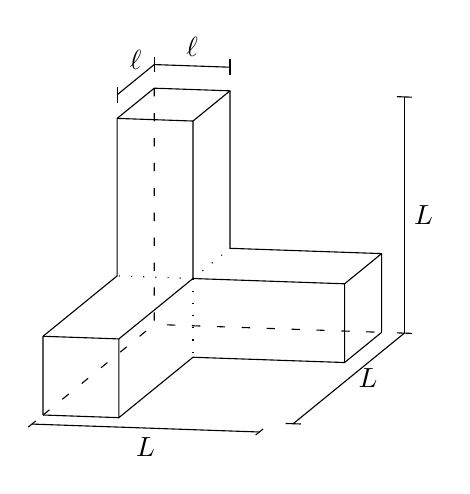
\begin{tikzpicture}[rotate around y = -5]

    % Frente
    \draw (3,0,0) -- (3,1,0) -- (1,1,0) -- (1,3,0) -- (0,3,0);
    \draw (0,3,0) -- (0,3,1) -- (0,1,1) -- (0,1,3) -- (0,0,3);
    \draw (0,3,1) -- (1,3,1) -- (1,1,1) -- (1,1,3) -- (0,1,3);
    \draw (1,1,3) -- (1,0,3) -- (1,0,1) -- (3,0,1) -- (3,0,0);
    \draw (3,0,1) -- (3,1,1) -- (1,1,1);
    \draw (0,0,3) -- (1,0,3);
    \draw (1,3,1) -- (1,3,0);
    \draw (3,1,0) -- (3,1,1);
    
    \draw[loosely dotted] (1,1,1) -- (1,1,0);
    \draw[loosely dotted] (1,1,1) -- (1,0,1);
    \draw[loosely dotted] (1,1,1) -- (0,1,1);
    
    % trás
    \draw[loosely dashed] (0,3,0) -- (0,0,0) -- (3,0,0);
    \draw[loosely dashed] (0,0,3) -- (0,0,0);
    
    % Medidas
    \draw (3.2,0,0) -- (3.4,0,0);
    \draw (3.2,0,3) -- (3.4,0,3);
    \draw (3.3,0,0) -- node[right]{$L$} (3.3,0,3);
    
    \draw (3.3,0,0) -- node[right]{$L$} (3.3,3,0);
    \draw (3.2,3,0) -- (3.4,3,0);
    
    \draw (0,0,3.2) -- (0,0,3.4);
    \draw (3,0,3.2) -- (3,0,3.4);
    \draw (0,0,3.3) -- node[below]{$L$} (3,0,3.3);
    
    \draw (0,3.2,0) -- (0,3.4,0);
    \draw (1,3.2,0) -- (1,3.4,0);
    \draw (0,3.3,0) -- node[above]{$\ell$} (1,3.3,0);
    \draw (0,3.2,1) -- (0,3.4,1);
    \draw (0,3.3,1) -- node[above]{$\ell$}(0,3.3,0);
    
\end{tikzpicture}
\caption{Objeto formado pela junção de três prismas quadrados de comprimento $L$ e laterais $\ell$. As linhas tracejadas representam as arestas na parte de trás do objeto, enquanto as linhas pontilhadas representam as arestas formadas pela inserseção de duas faces dianteiras. \label{Fig:CMObj3D}}
\end{marginfigure}

\noindent{}Dividindo o corpo em partes e utilizando argumentos de simetria, determinamos que os centros de massa das partes estão localizados nas seguintes posições:
\begin{align}
    \vec{r}_1 &= \nicefrac{\ell}{2}\;\versi + 2\ell\;\versj + \nicefrac{\ell}{2}\;\versk \\
    \vec{r}_2 &= \nicefrac{\ell}{2}\;\versi + \nicefrac{\ell}{2}\;\versj + 2\ell\;\versk \\
    \vec{r}_3 &= \nicefrac{3\ell}{2}\;\versi + \nicefrac{\ell}{2}\;\versj + \nicefrac{\ell}{2}\;\versk.
\end{align}
%
Os volumes de cada parte são dados por
\begin{align}
    V_1 &= 2\ell^3\\
    V_2 &= 2\ell^3\\
    V_3 &= 3\ell^3,
\end{align}
%
totalizando $7\ell^3$.

\begin{marginfigure}[-10cm]
\centering
\begin{tikzpicture}[rotate around x = 15]
    % eixos
    \draw[-Stealth, loosely dashed] (0,0,0) -- (4,0,0) node[below left] {$x$};
    \draw[-Stealth, loosely dashed] (0,0,0) -- (0,4,0) node[below left] {$y$};
    \draw[-Stealth, loosely dashed] (0,0,0) -- (0,0,4) node[below right] {$z$};

    % Frente
    \draw (3,0,0) -- (3,1,0) -- (1,1,0) -- (1,3,0) -- (0,3,0);
    \draw (0,3,0) -- (0,3,1) -- (0,1,1) -- (0,1,3) -- (0,0,3);
    \draw (0,3,1) -- (1,3,1) -- (1,1,1) -- (1,1,3) -- (0,1,3);
    \draw (1,1,3) -- (1,0,3) -- (1,0,1) -- (3,0,1) -- (3,0,0);
    \draw (3,0,1) -- (3,1,1) -- (1,1,1);
    \draw (0,0,3) -- (1,0,3);
    \draw (1,3,1) -- (1,3,0);
    \draw (3,1,0) -- (3,1,1);
       
    % planos de simetria e CM
    \draw[dotted] (0,2,0) -- (0,2,1) -- (1,2,1) -- (1,2,0) -- cycle;
    \draw[dotted] (0.5,3,0) -- (0.5,3,1) -- (0.5,1,1) -- (0.5,1,0) -- cycle;
    \draw[dotted] (0,3,0.5) -- (0,1,0.5) -- (1,1,0.5) -- (1,3,0.5) -- cycle;
    \draw[fill] (0.5, 2, 0.5) circle (1pt);
    
%    \draw[dotted] (1.5,0,0) -- (1.5,1,0) -- (1.5,1,1) -- (1.5,0,1) -- cycle;
%    \draw[dotted] (0,0.5,0) -- (3,0.5,0) -- (3,0.5,1) -- (0,0.5,1) -- cycle;
%    \draw[dotted] (0,0,0.5) -- (0,1,0.5) -- (3,1,0.5) -- (3,0,0.5) -- cycle;
    \draw[fill] (1.5,0.5,0.5) circle (1pt);
    
%    \draw[dotted] (0,0,2) -- (0,1,2) -- (1,1,2) -- (1,0,2) -- cycle;
%    \draw[dotted] (0.5,0,1) -- (0.5,1,1) -- (0.5,1,3) -- (0.5,0,3) -- cycle;
%    \draw[dotted] (0,0.5,3) -- (0,0.5,1) -- (1,0.5,1) -- (1,0.5,3) -- cycle;
    \draw[fill] (0.5,0.5,2) circle (1pt);
    
    % cortes
    \draw[dashdotted] (1,1,1) -- (1,1,0) -- (0,1,0) -- (0,1,1) -- cycle;
    \draw[dashdotted] (1,1,1) -- (1,0,1) -- (0,0,1) -- (0,1,1);
    
    % sombra
    \path[pattern = north west lines, pattern color = lightgray] (0,1,0) -- (0,1,1) -- (3,1,1) -- (3,1,0) -- cycle;
    \path[pattern = north east lines, pattern color = lightgray] (0,1,1) -- (0,0,1) -- (3,0,1) -- (3,1,1) -- cycle;
    \path[pattern = north west lines, pattern color = lightgray] (3,1,1) -- (3,0,1) -- (3,0,0) -- (3,1,0) -- cycle;
    
    % rótulos
    \node[draw, circle, scale = 0.7] (P1) at (1,3.3,0) {$1$};
    \node[draw, circle, scale = 0.7] (P2) at (-0.3,1,2.5) {$2$};
    \node[draw, circle, scale = 0.7] (P3) at (2.75,1.3,0) {$3$};
    
\end{tikzpicture}
\caption{Dividimos o objeto em três paralelepípedos, permitindo que determinemos as posições do centro de massa de cada parte através da simetria (para simplificar a figura, mostramos os planos de simetria somente para uma das partes). Verifique que temos um paralelepípedo maior, disposto ao longo do eixo $x$. As linhas ponto-tracejadas mostram os planos de corte para a divisão. \label{Fig:CMObj3DCortado}}
\end{marginfigure}

Utilizando a Expressão~\eqref{Eq:CMDensVolConst}, podemos determinar a posição do centro de massa:
\begin{align}
    \vec{r}_{CM} &= \frac{1}{7\ell^3} [(2\ell^3)(\nicefrac{\ell}{2}\;\versi + 2\ell\;\versj + \nicefrac{\ell}{2}\;\versk) \\
    &\phantom{=\frac{1}{7\ell^3} [} + (2\ell^3)(\nicefrac{\ell}{2}\;\versi + \nicefrac{\ell}{2}\;\versj + 2\ell\;\versk) \\
    &\phantom{=\frac{1}{7\ell^3} [} + (3\ell^3)(\nicefrac{3\ell}{2}\;\versi + \nicefrac{\ell}{2}\;\versj + \nicefrac{\ell}{2}\;\versk)] \\
    &= \frac{1}{7\ell^3} [(\ell^4 + \ell^4 + \nicefrac{9\ell^4}{2})\versi \\
    &\phantom{=\frac{1}{7\ell^3} [}+ (4\ell^4 + \ell^4 + \nicefrac{3\ell^4}{2})\versj \\
    &\phantom{=\frac{1}{7\ell^3} [}+ (\ell^4 + 4\ell^4 + \nicefrac{3\ell^4}{2})\versk,
\end{align}
%
Finalmente,
\begin{equation}
	\vec{r}_{CM} = \np{0,9286} \ell\; \versi + \np{0,9286} \ell \; \versj + \np{0,9286} \ell \; \versk.
\end{equation}
%
Observe que o resultado é igual para todos os eixos: existem três planos que são capazes de dividir o corpo em partes simétricas, sendo que o encontro dos três se dá no eixo que passa exatamente no meio do octante formado pelos eixos $x$, $y$ e $z$ --~veja a linha tracejada na Figura~\ref{Fig:CMObj3DPosicaoCM}~--. Talvez, numa análise instintiva, pudessemos acreditar que o centro de massa estivesse mais afastado da origem, fora do corpo. Uma maneira de perceber o contrário é imaginar um plano a uma altura $y = \ell$: percebemos que a maior parte da massa está abaixo desse plano, portanto o centro de massa também deve estar abaixo do plano. Porém, por simetria, o centro de massa deve estar localizado sobre a reta tracejada. Logo, ele deve estar mais próximo da origem que o ponto $P = \ell \; \versi + \ell \; \versj + \ell \; \versk$ que é a interseção entre o plano $y = \ell$ e a reta. 

\begin{marginfigure}[-5cm]
\centering
\begin{tikzpicture}[rotate around y = 10, rotate around z = -3]
	% eixos
    \draw[-Stealth] (3,0,0) -- (3.5,0,0) node[below left] {$x$};
    \draw[-Stealth] (0,3,0) -- (0,4,0) node[below left] {$y$};
    \draw[-Stealth] (0,0,3) -- (0,0,4) node[below right] {$z$};


    
	% Plano de simetria
	\path[pattern = north west lines, pattern color = lightgray] (0,0,0) -- (0,3.5,0) -- (3,3.5,3) -- (3,0,3) -- cycle;
	\draw[gray] (1,0,1) -- (3,0,3) -- (3,3.5,3) -- (0,3.5,0);

	\draw[pattern = north west lines, pattern color = gray, thick] (0,3,0) -- (1,3,1) -- (0,3,1) -- cycle;
	\draw[pattern = north west lines, pattern color = gray, thick] (1,3,1) -- (0,3,1) -- (0,1,1) -- (1,1,1) -- cycle;
	\draw[pattern = north west lines, pattern color = gray, thick] (1,1,1) -- (0,1,1) -- (0,1,3) -- (1,1,3) -- cycle;
	\draw[pattern = north west lines, pattern color = gray, thick] (0,1,3) -- (1,1,3) -- (1,0,3) -- (0,0,3) -- cycle;
    \draw[pattern = north west lines, pattern color = gray, thick] (1,1,1) -- (1,0,1) -- (1,0,3) -- (1,1,3) -- cycle;

	\draw[pattern = north east lines, pattern color = lightgray] (0,3,0) -- (1,3,0) -- (1,3,1);
	\draw[pattern = north east lines, pattern color = lightgray] (1,3,1) -- (1,3,0) -- (1,1,0) -- (1,1,1) -- cycle;
	\draw[pattern = north east lines, pattern color = lightgray] (1,1,1) -- (1,1,0) -- (3,1,0) -- (3,1,1) -- cycle;
	\draw[pattern = north east lines, pattern color = lightgray] (3,1,0) -- (3,1,1) -- (3,0,1) -- (3,0,0) -- cycle;
	\draw[pattern = north east lines, pattern color = lightgray] (1,1,1) -- (1,0,1) -- (3,0,1) -- (3,1,1) -- cycle;

	\draw[thick] (0,3,0) -- (1,3,1) -- (1,0,1);
	\draw[dashed, thick] (0,0,0) -- (0,3,0);
	\draw[dashed, thick] (0,0,0) -- (0,0,3);
	\draw[dashed, thick] (0,0,0) -- (3,0,0);
	\draw[dashed, thick] (0,0,0) -- (1,0,1);

	\draw[thick, dashdotted] (0,0,0) -- (3,3,3);
	% CM
	\draw[-Stealth, very thick] (0,0,0) -- (0.9286,0.9286,0.9286);
	\draw[fill] (0.9286,0.9286,0.9286) circle (1pt) node[below right]{CM};

\end{tikzpicture}
\caption{Podemos dividir o objeto simetricamente ao realizarmos cortes como o mostrado na figura acima, um para cada eixo. Tais planos determinam uma reta que passa pela origem (reta ponto-tracejada). O vetor denota a posição do centro de massa. \label{Fig:CMObj3DPosicaoCM}}
\end{marginfigure}


%%%%%%%%%%%%%%%%%%%%%%%%%%%%%%%%%%%%%%%%%%%%%%%%%%
%\paragraph{Exemplo: Massa negativa/soma-subtração}
%%%%%%%%%%%%%%%%%%%%%%%%%%%%%%%%%%%%%%%%%%%%%%%%%%

%\textbf{Exemplo com massa negativa, ou soma e subtração (lembrar do exemplo de um livro em que se extrai uma região circular de um circulo maior}

%%%%%%%%%%%%%%%%%%%%%%%%%%%%%%%%%%%%%%%%
%\paragraph{Centro de massa de uma barra} % tirar
%%%%%%%%%%%%%%%%%%%%%%%%%%%%%%%%%%%%%%%%

%Podemos calcular o centro de massa de uma barra fina e de densidade homogênea se a dividirmos em $n$ ``fatias'' finas. Como essas fatias são finas, podemos considerar que o centro de massa fica localizado no meio da fatia (e podemos aumentar o número de fatias arbitrariamente caso essa aproximação seja ruim, mas veremos que ela não é). Nesse caso, podemos dizer que para o eixo $x$
%\begin{equation}
%  x_{CM} = \frac{1}{M_t} \sum x_i m_i
%\end{equation}
%
%Se todas as fatias têm a mesma massa $m$, temos
%\begin{equation}
%  x_{CM} = \frac{m}{M_t} \sum x_i.
%\end{equation}
%
%Também podemos verificar que $M_t = n m$. Logo
%\begin{equation}
%  x_{CM} = \frac{1}{n} \sum x_i.
%\end{equation}
%
%A equação acima não passa de uma média das posições das fatias. Podemos pensar da seguinte forma: para uma fatia localizada a uma distância $a$ da origem, temos uma outra localizada a uma distância $a$ da extremidade oposta. Se a barra tem comprimento $L$, então a contribuição dessas duas para o somatório da equação acima é
%\begin{equation}
%  \sum x_i = (a) + (L - a) + \dots,
%\end{equation}
%
%o que claramente resultará em
%\begin{equation}
%  \sum x_i = \frac{n}{2}L,
%\end{equation}
%
%pois se temos $n$ fatias, temos $n/2$ pares de fatias. Consequentemente
%\begin{equation}
%  x_{CM} = \frac{L}{2}.
%\end{equation}

%%%%%%%%%%%%%%%%%%%%%%%%%%%%%%%%%%%%%%%%%%%%%%%%%%%%%%%%%%%%%%%%%%%%
\subsection{Centro de massa de uma distribuição arbitrária de massa}
%%%%%%%%%%%%%%%%%%%%%%%%%%%%%%%%%%%%%%%%%%%%%%%%%%%%%%%%%%%%%%%%%%%%

% https://tex.stackexchange.com/questions/123158/tikz-using-the-ellipse-command-with-a-start-and-end-angle-instead-of-an-arc
\tikzset{
    partial ellipse/.style args={#1:#2:#3}{
        insert path={+ (#1:#3) arc (#1:#2:#3)}
    }
}

\begin{marginfigure}
\centering
\begin{tikzpicture}[interface/.style={
        % superfície
        postaction={draw,decorate,decoration={border,angle=-45,
                    amplitude=0.2cm,segment length=2mm}}},
    ]

% laterais
\draw (0,0) -- (-1.3,-3);
\draw (1.3,-3) -- (0,0);  

% fundo
\draw[dotted] (-1.28,-3) arc (180:360:1.28 and -0.53);
\draw (-1.3,-3) arc (180:360:1.3 and 0.55);
\draw[fill] (0,-3) circle (0.6pt);

% Eixos
% x
\draw[dotted] (0,-3) -- +(15:-1.15);
\draw[dashdotted,-Stealth] (0,-3) +(15:-1.15) -- +(15:-2) node[below right]{$x$};
\draw[fill](0,-3) +(15:-1.14) circle (0.6pt);
\draw[dotted] (0,-3) -- +(15:1.15);
\draw[dashdotted] (0,-3) +(15:1.15) -- +(15:2);
\draw[fill](0,-3) +(15:1.125) circle (0.6pt);

% y
\draw[dotted] (0,-3) -- +(-15:-1.15);
\draw[dashdotted] (0,-3) +(-15:-1.15) -- +(-15:-2);
\draw[fill](0,-3) +(-15:-1.125) circle (0.6pt);
\draw[dotted] (0,-3) -- +(-15:1.15);
\draw[dashdotted, -Stealth] (0,-3) +(-15:1.15) -- +(-15:2) node[below left]{$y$};
\draw[fill](0,-3) +(-15:1.14) circle (0.6pt);

%
% z
\draw[dashdotted,-Stealth] (0,0) -- (0,0.75) node[below left]{$z$};
\draw[loosely dotted] (0,-3.55) -- (0,0);
\draw[dashdotted] (0,-3.55) -- (0,-4);

\draw[fill] (0,-2.25) circle (1pt) node[above right] {CM};

\begin{scope}[scale = 0.2, shift = {(-2,-12)}]
    \draw[fill, lightgray, draw = black] (1,1,1) -- (1,1,0) -- (0,1,0) -- (0,1,1) -- cycle;
    \draw[fill, lightgray, draw = black] (1,1,1) -- (0,1,1) -- (0,0,1) -- (1,0,1) -- cycle;
    \draw[fill, lightgray, draw = black] (1,1,1) -- (1,1,0) -- (1,0,0) -- (1,0,1) -- cycle;
\end{scope}

\draw[-Stealth] (0,-3) -- node[right]{$\vec{r}_{\rm{CM}}^{R_i}$} (-0.35,-2.38);
\draw[fill] (-0.35,-2.38) circle (0.6pt);

\end{tikzpicture}
\caption{Para determinar a posição do centro de massa de um cone, podemos dividí-lo em diversos cubos e determinar a posição do centro de massa do conjunto de cubos. \label{Fig:CMDiscretizacaoObjeto3D}}
\end{marginfigure}

A princípio, podemos utilizar a expressão~\eqref{Eq:CMConjuntoDeParticulas} para determinar o centro de massa de qualquer corpo, desde que possamos somar a contribuição de todas as partículas que compõe o corpo. Claramente, no entanto, isso não é nada prático. 

Se o objeto tem formas complexas, podemos realizar uma divisão em regiões cujos centros de massa possamos determinar por argumentos de simetria, como fizemos nas seções anteriores. Porém, nem sempre uma divisão em cubos é efetiva. Uma maneira alternativa consiste em dividir o corpo em $N$ pequenos cubos contendo diversas partículas, sendo que cada cubo tem massa $M_{R_i}$ --~como no caso do cone da Figura~\ref{Fig:CMDiscretizacaoObjeto3D}~--. Claramente uma divisão em cubos não é a melhor escolhar para descrever um cone, porém se eles forem pequenos o suficiente, teremos uma aproximação razoável. Esse tipo de procedimento pode ser implementado em programas de computador com certa facilidade, e podem até mesmo considerar situações onde a massa não é homogênea, já que determinamos a massa de cada cubo individualmente.

Se tomarmos cubos extremamente pequenos, temos uma soma que tende a infinitos termos. Esse processo é a própria definição de uma uma integral em duas ou três dimensões sobre a área ou volume no qual se distribui a massa:
\begin{align}\label{Eq:CMDistContinua}
  \vec{r}_{\textrm{CM}} &= \lim_{N \to \infty} \frac{1}{M} \sum_{i = 1}^N M_{R_i} \vec{r}_{\rm{CM}}^{R_i} \\
  &= \frac{1}{M} \int \vec{r} \; dm, \mathnote{Centro de Massa de uma distribuição contínua de massa}
\end{align}
%
onde $dm$ representa a massa \emph{infinitesimal} associada a um cubo quando fazemos o número de cubos tendendo ao infinito e $M$ representa a massa total do corpo. Esse resultado pode ser interpretado de uma maneira mais simples se considerarmos que o elemento de massa está relacionado à densidade e ao volume do elemento de massa através de $dm = \rho(\vec{r}) \; dV$. Logo, basta considerarmos uma integral na região do espaço ocupada pelo corpo.

Da mesma forma que na integral em uma dimensão, a ideia não é determinar o resultado desse limite, mas substituir o problema por um equivalente e que nos permita determinar o centro de massa. Matematicamente, o processo de resolução de uma integral em duas ou três dimensões consiste em resolver duas ou três integrais unidimensionais, respectivamente. A principal diferença é a de que os limites de integração não são números, mas funções que descrevem as superfícies externas da região do espaço onde estamos realizando a integração, o que no nosso caso é a própria superfície externa do corpo.


A expressão acima pode ser considerada a forma mais geral de se determinar o centro de massa para uma distribuição contínua de massa, pois a discussão anterior sobre discretização pode ser interpretada como uma simples propriedade da integral acima. Muitas vezes não é necessário considerar o caso tridimensional, bastando substituir $dm = \sigma(\vec{r}) \; dA$ ou $dm = \lambda(x) \; dx$ --~onde $\sigma(\vec{r})$ e $\lambda(x)$ representam as densidades superficial de massa e a densidade linear de massa (respectivamente), e $dA$ e $dx$ correspondem aos elementos de área e de comprimento~--.

Mesmo assumindo um conhecimento sólido de cálculo, a definição dada pela Equação~\eqref{Eq:CMDistContinua} não é extremamente útil: Precisamos poder descrever a forma do objeto matematicamente, o que só é fácil para formas relativamente simples. De qualquer maneira, para algumas formas (cones e pirâmides, por exemplo) e no caso de termos uma densidade que possa ser calculada para cada ponto do espaço através de uma função, a forma integral é bastante útil.

%%%%%%%%%%%%%%%%%%%%%%%%%%%%%%%%%%%%%%%%%%%%%%%%%%
\subsection{Movimento do centro de massa}
%%%%%%%%%%%%%%%%%%%%%%%%%%%%%%%%%%%%%%%%%%%%%%%%%%

Imagine que um projétil seja lançado com velocidade $\vec{v}_0$ fazendo um ângulo $\theta$ com a horizontal. Em um determinado momento, o projétil explode. Sabemos de nosso estudo de cinemática que a trajetória do projétil é uma parábola até o momento da detonação. Sabemos que um projétil não é uma partícula, porém toda a descrição dada para o movimento assume que sim, isto é, na verdade o que fizemos foi descrever a trajetória do centro de massa. O que acontece com a trajetória do centro de massa após a explosão?

Cada uma das partículas que compunham o projétil serão sujeitas a forças muito intensas durante a explosão. Isso alterará a trajetória de cada uma delas. Para determinar a trajetória do centro de massa, devemos verificar através da Equação~\eqref{Eq:SegundaLeiSistemaDeParticulasMConst} qual é a aceleração a que o centro de massa estará sujeito. Sabemos que a força externa resultante sobre as partículas após a explosão será simplesmente\footnote{Estamos desprezando o efeito da força de arrasto.} a força peso de cada uma delas, o que implica em uma força peso igual àquela do projétil antes da explosão:
\begin{align}
	\vec{F}_{R}^{\rm{ext}} &= \sum_i^N \vec{F}_g^i \\
		&= \vec{F}_g.
\end{align}
%
Além disso, sabemos que a velocidade do centro de massa não é alterada por forças internas, somente por forças externas:
\begin{align}
	\vec{F}_R^{\rm{ext}} &= \frac{d}{dt}\vec{P} \\
		&= m\frac{d}{dt}\vec{v}_{\rm{CM}}.
\end{align}
%
O fato de que as forças durante a explosão são internas implica então em uma igualdade entre a velocidade do centro de massa antes e depois da explosão, pois a aceleração do centro de massa é nula. Logo, se a velocidade do centro de massa não é alterada, e ele continua sujeito à mesma força após a explosão, concluímos que \emph{a desintegração do projétil não altera a trajetória do centro de massa}.

\begin{marginfigure}
\centering
\begin{tikzpicture}[>=Stealth, decoration=bumps]
    \draw[->] (0,0) -- (4,0) node[below left]{$x$};
    \draw[->] (0,0) -- (0,2) node[below left]{$y$};
    
    \draw[smooth, samples=1000, domain=0:2.33] plot (\x, {2*\x - 0.6*\x*\x});
    \draw[densely dotted, smooth, samples=1000, domain=2.33:3.33] plot (\x, {2*\x - 0.6*\x*\x});
    
    \coordinate (O) at (0,0);
    \coordinate (A) at (1,0);
    \coordinate (B) at (63.434948823:1);
       
	\draw[->, thick] (0,0) -- (63.43:1.5) node[above]{$\vec{v}_0$};
    \pic [draw, "$\theta$", angle eccentricity=1.5] {angle = A--O--B};

	\draw[decorate] (2.33, 1.4) circle (2mm);
        
\end{tikzpicture}
\caption{Em uma explosão, as forças efetuadas sobre as várias partes do corpo que explode são internas. Nesse caso, o movimento do centro de massa não é afetado.\label{Fig:ExplosaoProjetil}}
\end{marginfigure}


% problema do projétil num lançamento obliquo que explode em duas partes

% exemplo clássico de uma pessoa que se move em um barco: tanto o barco quanto a pessoa se movem e o CM permanece no mesmo lugar.

%%%%%%%%%%%%%%%%%%%%%%%%%%%%%%%%%%%%%%%
\section{Conservação do momento linear}
%%%%%%%%%%%%%%%%%%%%%%%%%%%%%%%%%%%%%%%

A partir da Expressão~\eqref{Eq:SegundaLeiSistemaDeParticulas} para a Segunda Lei de Newton, juntamente com a Expressão~\eqref{Eq:MomentoLinearSistemaDeParticulas} para o momento linear de um sistema de partículas, podemos determinar uma \emph{lei de conservação}.

Sabemos que a definição de um sistema é arbitrária. Nesse caso, podemos o escolher de maneira que a \emph{a força resultante externa seja nula}. Nesse caso, temos que o momento linear do sistema de partículas deve se manter constante, já que
\begin{equation}
	\vec{F}_R^{\rm{ext}} = \frac{d}{dt} \vec{P}.
\end{equation}
%
Isso significa que \emph{se a força resultante externa é zero, então o momento linear total do sistema se mantém constante, não importando que interações aconteçam entre as partículas}. Consequentemente, entre dois instantes inicial $i$ e final $f$ quaisquer, temos que:
\begin{equation}\label{Eq:ConservacaoMomentoLinear}
	\vec{P}_{\rm{CM}}^i = \vec{P}_{\rm{CM}}^f. \mathnote{Princípio da conservação do momento linear}
\end{equation}

A expressão acima é extremamente relevante pois é muito comum que possamos definir um sistema de maneira que a força resultante externa seja nula. A conservação do momento linear nos fornece um valor cujo cálculo é simples e descreve uma característica do sistema como um todo. Além disso, como o momento linear do sistema é dado pela soma dos momentos lineares das diversas partículas que o compôe, temos uma relação entre os momentos de tais partículas. De uma maneira geral, podemos traçar um paralelo com a conservação da energia, e podemos afirmar que o fato de que o momento linear se conservar nos permite a obtenção de variáveis em um sistema sem a necessidade de entender quais são as minúcias de cada interação entre as partículas do sistema.

Na Figura~\ref{Fig:ExplosaoProjetil} verificamos que se um projétil explode durante um movimento parabólico, o centro de massa continua a descrever a trajetória inicial. Se considerarmos uma situação em que a força externa é nula --~a explosão do mesmo projétil no espaço, longe de qualquer planeta, por exemplo~--, verificamos através da Expressão~\ref{Eq:ConservacaoMomentoLinear} que o momento linear antes e depois da explosão devem ter o mesmo valor, pois a força resultante externa é nula. Se fixarmos o sistema de referência na posição do próprio projétil, temos que o momento linear inicial é nulo, logo
\begin{align}
    \vec{P}_{\rm{CM}}^i &= \vec{P}_{\rm{CM}}^f \\
    0 &= \vec{P}_{\rm{CM}}^f.
\end{align}
%
Lembrando que podemos separar uma relação vetorial em três eixos, temos que
\begin{equation}
\begin{system}
    p_{1,f}^x + p_{2,f}^x + p_{3,f}^x + \dots &= 0 \\
    p_{1,f}^y + p_{2,f}^y + p_{3,f}^y + \dots &= 0 \\
    p_{1,f}^z + p_{2,f}^z + p_{3,f}^z + \dots &= 0,
\end{system}
\end{equation}
%
onde usamos a Equação~\ref{Eq:MomentoLinearSistemaDeParticulas} para escrever o momento linear do sistema como a soma dos momentos lineares de cada partícula. As equações acima nos dão informações que relacionam os diversos momentos lineares das partículas e, em diversas situações, podemos utilizar tais relações, juntamente com algum conhecimento prévio de algumas variáveis para determinar o valor de outra variável que desejamos conhecer.

Devemos observar que o momento linear e a velocidade são grandezas vetoriais, por isso as velocidades na expressão~\eqref{Eq:ConservacaoMomentoUnidimensional} devem ter sinais apropriados conforme seus sentidos sejam  no sentido positivo ou negativo do eixo de referência adotado. Note que a escolha do sentido positivo é arbitrária, porém uma vez escolhido, devemos escrever as velocidades de maneira coerente. Finalmente, os resultados obtidos para a velocidade poderão ser positivos ou negativos, sendo que valores negativos implicam simplesmente em velocidades no sentido negativo do eixo.

%%%%%%%%%%%%%%%%%%%%%%%%%%%%%%%%%%%%%%%%%%%%%%%%%%%%%%%%
\paragraph{Exemplo: Explosão de um corpo em três partes}
%%%%%%%%%%%%%%%%%%%%%%%%%%%%%%%%%%%%%%%%%%%%%%%%%%%%%%%%

\begin{marginfigure}
\centering
\begin{tikzpicture}[>=Stealth]
    \draw[pattern = north west lines, pattern color = gray, draw = gray] (0,0) circle (0.3);
    \draw[dashdotted] (0,0)++(-0.3,0) -- +(-1.5,0);
    \draw[dashdotted, ->] (0,0) ++(0.3,0) -- +(1.5,0) node[below left]{$x$};
    \draw[dashdotted] (0,0) ++(0,-0.3) -- +(0,-1.5);
    \draw[dashdotted, ->] (0,0) ++(0,0.3) -- +(0,1.5) node[below left]{$y$};
    
    \draw[pattern = north west lines] (-1.2,0) circle (1.8mm);
    \draw[->] (-1.38,0) -- node[above]{$\vec{v}_1$} +(-1,0);
    
    \draw[pattern = north west lines] (17.42:1.07) circle (2.1mm);
    \draw[->] (17.42:1.28) -- node[above]{$\vec{v}_2$} +(17.42:0.89);
    
    \draw[pattern = north west lines] (-74.62:0.5) circle (1.5mm);
    \draw[->] (-74.62:0.65) -- node[right]{$\vec{v}_3$} +(-74.62:0.61);
\end{tikzpicture}
\caption{Explosão de um corpo em três partes.}
\end{marginfigure}

Como exemplo da aplicação do princípio de conservação do momento linear, vamos considerar a explosão de um corpo que se encontra em repouso sobre uma mesa. Inicialmente o corpo se encontra em repouso em relação a um sistema de coordenadas fixado na mesa e após a explosão se divide em três partes, cujas velocidades são:
\begin{align}
    \vec{v}_1 &= -\np[m/s]{3.0} \versi\\
    \vec{v}_2 &= \np[m/s]{2.55} \versi + \np[m/s]{0.8} \versj \\
    \vec{v}_3 &= \np[m/s]{0.33} \versi - \np[m/s]{1.2} \versj.
\end{align}
%
Se a massa do fragmento 1 é $m_1 = \np[kg]{0,25}$, quais são as massas dos fragmentos 2 e 3?

\begin{marginfigure}
\centering
\begin{tikzpicture}[>=Stealth,
interface/.style={
        % superfície
        postaction={draw,decorate,decoration={border,angle=-45,
                    amplitude=0.2cm,segment length=2mm}}}
                    ]
                    
    \draw[interface] (-2,0) -- (2,0);
    
    \draw[pattern = north west lines] (-0.5,0) rectangle (0.5,0.5);
    \draw[fill] (0, 0.25) circle (1pt);
    \draw[->, thick] (0, 0.25) --+(0,-1) node[right]{$\vec{P}$};
    \draw[->, thick] (0, 0.5) -- +(0,1) node[right]{$\vec{N}$};
\end{tikzpicture}
\caption{Apesar de termos forças externas atuando sobre o corpo, a força resultante externa é nula. Portanto, temos que o momento linear do sistema se mantém constante.}
\end{marginfigure}

Sabemos que o corpo inicialmente está sobre uma mesa e está em repouso. Nesse caso, sabemos que ele está sujeito a uma força normal e à força peso. No entanto, como não há aceleração no sistema, sabemos que as forças devem estar em equilíbrio. Nesse caso, não há nenhuma força externa resultante atuando sobre o sistema, portanto podemos utilizar a conservação do momento linear:
\begin{equation}
    \vec{P}_{\rm{CM}}^i = \vec{P}_{\rm{CM}}^f.
\end{equation}
%
O momento linear inicial do sistema está relacionado à velocidade do centro de massa,
\begin{equation}
    \vec{P}_{\rm{CM}} = m \vec{v}_{\rm{CM}},
\end{equation}
%
assim como à soma dos momentos lineares das partículas que compõe o sistema:
\begin{equation}
    \vec{P}_{\rm{CM}} = \sum_i \vec{p}_i.
\end{equation}
%
Sabemos que antes da explosão, o corpo estava em repouso em relação à mesa, por isso temos que o a velocidade do centro de massa em relação à mesa é zero. Por outro lado, sabemos que o momento linear do centro de massa após a explosão é dado pela soma dos momentos lineares das partículas. Utilizando a conservação do momento linear, obtemos
\begin{equation}
    \sum_i \vec{p}_i = 0.
\end{equation}
%
Separando tal relação em três eixos e considerando que só temos três partículas após a explosão, obtemos
\begin{equation}
\begin{system}
    p_1^x + p_2^x + p_3^x &= 0 \\
    p_1^y + p_2^y + p_3^y &= 0,
\end{system}
\end{equation}
%
ou, utilizando $p_x = m v_x$ e $o_y = mv_y$,
\begin{equation}
\begin{system}
    m_1v_1^x + m_2 v_2^x + m_3 v_3^x &= 0 \\
    m_1v_1^y + m_2 v_2^y + m_3 v_3^y &= 0.
\end{system}
\end{equation}
%
Substituindo os valores das velocidades, obtemos duas equações que envolvem as massas:
\begin{equation}
\begin{system}
    -3 \,m_1 + \np{2.55} \,m_2 + \np{0.33} \,m_3 &= 0 \\
    0 \,m_1 + \np{0.8} \,m_2 - \np{1.2} \,m_3 &= 0,
\end{system}
\end{equation}
%
sendo que as soluções são
\begin{align}
    m_2 &= \np[kg]{0.271} \\
    m_3 &= \np[kg]{0.181}.
\end{align}

%%%%%%%%%%%%%%%%%%
\section{Colisões}
%%%%%%%%%%%%%%%%%%

Podemos empregar a conservação do momento linear para discutir colisões. Uma colisão é caracterizada pela interação de dois corpos através forças de contato entre as suas superfícies, isto é, \emph{forças normais e de atrito}. Na Figura~\ref{Fig:ColisaoEntreDoisDiscos} mostramos uma colisão bidimensional entre dois discos. Vamos assumir que o disco da direita se encontra em repouso\footnote{Sempre podemos escolher um referêncial que satisfaça essa suposição em uma colisão entre dois corpos, bastando fixar o referecial no centro de massa de um dos corpos.}, enquanto o da esquerda se move para a direita com velocidade $\vec{v}$. Como poderíamos determinar o movimento dos discos após a colisão, dados os valores de massa e velocidade do disco incidente?

\begin{figure}[!h]\forcerectofloat
\centering
\begin{tikzpicture}[>=Stealth]

    \draw[pattern = north west lines] (-4.5,0.707) circle (0.5);
    \draw[thick, ->] (-4,0.707) -- node[above]{$\vec{v}$} +(1,0);
    \draw[dotted] (-4,0.707) -- +(6,0);
    
    \draw[pattern = north west lines, pattern color = gray, draw = gray] (-0.707,0.707) circle (0.5);
    \draw[pattern = north west lines] (0,0) circle (0.5);
    \draw[dashdotted, <-] (-0.3535,0.3535) +(45:2) node[below right]{$x$} -- +(225:2);
    \draw[dashdotted, <-] (-0.3535,0.3535) +(135:2) node[below left]{$y$} -- +(-45:2);
    
\end{tikzpicture}
\caption{Colisão bidimensional entre dois discos. \label{Fig:ColisaoEntreDoisDiscos}}
\end{figure}

A interação entre os discos de dá por meio de forças de contato que atuam no ponto onde os discos se tocam: no eixo $y$ mostrado na figura, temos a atuação de um par ação-reação de forças normais, enquanto no eixo $x$ temos a atuação de um par ação-reação de forças de atrito. Podemos considerar também que se esses discos se movem sobre uma mesa sem atrito, temos forças peso e normais atuando em cada corpo, perpendicularmente à figura. Supondo que não existe nenhuma aceleração no sistema, temos equilíbrio entre essas forças, e --~portanto~-- a força resultante externa é nula. Logo, podemos empregar a conservação do momento linear para determinar relações entre as componentes dos momentos lineares antes e depois da colisão:
\begin{equation}
\begin{system}
    p_{1,i}^x &= p_{1,f}^x + p_{2,f}^x \\
    p_{1,i}^y &= p_{1,f}^y + p_{2,f}^y.
\end{system}
\end{equation}
%
Apesar de termos encontrado uma relação entre os momentos lineares através da conservação do momento linear, não temos informações suficientes para a solução desse problema. Veremos adiante que algumas colisões mantém a energia cinética do sistema constante, o que nos daria mais uma relação entre as velocidades inicial e final dos discos. Outra possibilidade é a de termos um atrito desprezível no ponto de contato, o que faria com que as componentes das velocidades ao longo do eixo $x$ fossem constantes, afinal o impulso\footnote{Em uma colisão tal impulso é denominado como \emph{momento transferido} e é representado por $\vec{q} \equiv \Delta \vec{p}$.} responsável pela alteração do momento linear de cada disco seria somente ao longo do eixo $y$.

Nas próximas seções vamos tratar inicialmente algumas situações mais simples que a colisão discutida acima, restringindo o movimento a somente um eixo. Após isso, vamos discutir propriedades gerais de uma colisão e então retornaremos ao problema da colisão entre os dois discos.

%%%%%%%%%%%%%%%%%%%%%%%%%%%%%%%%%%%%%
\subsection{Colisões unidimensionais}
%%%%%%%%%%%%%%%%%%%%%%%%%%%%%%%%%%%%%

Uma colisão unidimensional é aquela em que dois corpos se aproximam com velocidades iniciais restritas a um eixo retilíneo, colidem, e se afastam com velocidades finais também restritas ao eixo retilíneo inicial (Figura~\ref{Fig:ColisaoUnidimensional}).

\begin{figure}[!h]
\centering
\begin{tikzpicture}[>=Stealth]
    \draw[dashdotted, ->] (-1.5,0) -- (6,0) node[below left]{$x$};
    
    \draw[fill] (1,0) circle (1mm);
    \draw[->] (1,0) -- node[above]{$\vec{v}_1^{\rm{ac}}$} +(1,0);
    
    \draw[fill] (3.5,0) circle (1mm);
    \draw[->] (3.5,0) -- node[above]{$\vec{v}_2^{\rm{ac}}$} +(-1,0);
    
    %%%
    
    \draw[dashdotted, ->] (-1.5,-1) -- (6,-1) node[below left]{$x$};
    
    \draw[fill] (2.5,-1) circle (1mm);
    \draw[fill] (2.7, -1) circle (1mm);
    
    %%%
    
    \draw[dashdotted, ->] (-1.5,-2) -- (6,-2) node[below left]{$x$};
    
    \draw[fill] (0.5,-2) circle (1mm);
    \draw[->] (0.5,-2) -- node[above]{$\vec{v}_1^{\rm{dc}}$} +(-1.6,0);
    
    \draw[fill] (3.2,-2) circle (1mm);
    \draw[->] (3.2,-2) -- node[above]{$\vec{v}_2^{\rm{dc}}$} +(0.4,0);
\end{tikzpicture}
\caption{Colisão unidimensional. \label{Fig:ColisaoUnidimensional}}
\end{figure}

Durante uma colisão, podemos considerar que o sistema está sujeito à condição de força resultante externa nula. Nesse caso, podemos afirmar para o problema mostrado na figura acima que
\begin{align}
    \vec{P}_{\rm{CM}}^i &= \vec{P}_{\rm{CM}}^f \\
    p_{1}^{\rm{ac}} + p_2^{\rm{ac}} &= p_{1}^{\rm{dc}} + p_{2}^{\rm{dc}} \\
    m_1 v_1^{\rm{ac}} + m_2 v_2^{\rm{ac}} &= m_1 v_1^{\rm{dc}} + m_2 v_2^{\rm{dc}}. \label{Eq:ConservacaoMomentoUnidimensional}
\end{align}
%
Se conhecermos o estado inicial de movimento --~isto é, as massas e as velocidades iniciais~-- a relação acima não determina completamente o estado final de movimento do sistema, porém nos dá condições de determinar qualquer uma das variáveis, dado que as outras sejam conhecidas.

De um ponto de vista energético, como temos que a força resultante externa é nula, sabemos que a energia do sistema é constante: se nenhuma força resultante atua sobre o sistema, o trabalho realizado sobre é necessariaemnte nulo. No entanto, não podemos garantir que a energia mecânica se conserve, pois podemos ter uma variação da energia interna dos corpos que colidem --~devido a deformações ou variação de temperatura, por exemplo~--. Veremos adiante que em algumas colisões, denominadas \emph{colisões elásticas}, poderemos assumir que a energia mecânica do sistema se conserve, porém esse não é o caso geral.

%%%%%%%%%%%%%%%%%%%%%%%%%%%%%%%%%%%%%%%%%%%%%%%%%%
\paragraph{Exemplo: Colisão entre bolas de bilhar}
%%%%%%%%%%%%%%%%%%%%%%%%%%%%%%%%%%%%%%%%%%%%%%%%%%

Assim como no caso da explosão de um corpo abordada anteriormente, podemos aplicar a conservação do momento linear à colisão unidimensional entre duas bolas de bilhar: novamente, o momento linear é conservado devido ao fato de que a força resultante externa é nula. Caso ambas as bolas se movam com velocidades iniciais
%
\begin{marginfigure}
\centering
\begin{tikzpicture}[>=Stealth, interface/.style={
        % superfície
        postaction={draw,decorate,decoration={border,angle=-45,
                    amplitude=0.2cm,segment length=2mm}}}]
    \draw[interface] (-2,-0.3) -- (2,-0.3);
    
    \draw[pattern = north west lines] (-0.3, 0) circle (0.3);
    \draw[pattern = north west lines] (0.3,0) circle (0.3);
    
    \draw[fill] (-0.3,0) circle (1pt);
    \draw[->, thick] (-0.3,0) -- +(0,-1) node[left]{$\vec{P}_1$};
    \draw[->, thick] (-0.3,0.3) -- +(0,1) node[left]{$\vec{N}_1$};
    
    \draw[fill] (0.3,0) circle (1pt);
    \draw[->, thick] (0.3,0) -- +(0,-1) node[right]{$\vec{P}_2$};
    \draw[->, thick] (0.3,0.3) -- +(0,1) node[right]{$\vec{N}_2$};
     
    
\end{tikzpicture}
\caption{Apesar de termos diversas forças além daquela que atua entre as duas bolas durante a colisão, a força resultante externa é igual a zero, o que garante que possamos utilizar a conservação de momento linear.}
\end{marginfigure}
%
\begin{align}
    v_1^{\rm{ac}} &= \np[m/s]{3,0} \\
    v_2^{\rm{ac}} &= -\np[m/s]{2,0}
\end{align}
%
e a velocidade final da partícula 1 seja
\begin{equation}
    v_1 = 0,
\end{equation}
%
qual é a velocidade da partícula 2 após a colisão, considerando que ambas têm a mesma massa?

Como temos o movimento de duas partículas somente em um eixo, podemos escrever
\begin{equation}
        m_1 v_1^{\rm{ac}} + m_2 v_2^{\rm{ac}} = m_1 v_1^{\rm{dc}} + m_2 v_2^{\rm{dc}}
\end{equation}
%
ou, considerando que ambas as massas são iguais,
\begin{equation}
        v_1^{\rm{ac}} + v_2^{\rm{ac}} = v_1^{\rm{dc}} + v_2^{\rm{dc}}
\end{equation}
%
o que resulta em
\begin{align}
    v_1^{\rm{ac}} + v_2^{\rm{ac}} &= v_1^{\rm{dc}} + v_2^{\rm{dc}} \\
    \np[m/s]{3,0} - \np[m/s]{2,0} &= 0 + v_2^{\rm{dc}}.
\end{align}
%
Finalmente,
\begin{equation}
    v_2^{\rm{dc}} = \np[m/s]{1,0}.
\end{equation}

%%%%%%%%%%%%%%%%%%%%%%%%%%%%%%%%%%%%%%%%
\paragraph{Discussão: Pêndulo balístico}
%%%%%%%%%%%%%%%%%%%%%%%%%%%%%%%%%%%%%%%%

Podemos utilizar a conservação do momento linear para determinarmos a velocidade de um projétil. A Figura~\ref{Fig:PenduloBalistico} mostra um pêndulo balístico, que consiste em um bloco/alvo suspenso. Quando o projétil atinge o alvo, devido à interação entre ambos a velocidade do projétil é diminuida até que ele pare, ficando alojado no bloco. Ao mesmo tempo, o bloco passa a ter uma velocidade final. Devido ao fato de que o alvo está suspenso, após a colisão o bloco se deslocará, efetuando um movimento de subida. A partir da distância percorrida verticalmente pelo alvo/bloco, podemos determinar a velocidade do projétil.

Durante a colisão, podemos considerar que o momento linear do sistema se conserva\footnote{Na verdade não temos um força resultante externa nula nesse sistema devido ao peso do projétil que não é equilibrado por nenhuma outra força. No entanto, discutiremos adiante que em alguns casos podemos desprezar o impulso de algumas forças, o que permite que possamos utilizar a conservação do moemnto linear.}. Por outro lado, devido às deformações do projétil e do alvo, não podemos considerar que a energia mecânica do sistema se mantenha constante\footnote{Enquanto no processo de explosão de um corpo discutido anteriormente temos um aumento da energia mecânica devido à liberação de energia interna do corpo, no presente caso temos que parte da energia mecânica do sistema é convertida em energia interna.}.

\begin{marginfigure}
\centering
\begin{tikzpicture}[>=Stealth, interface/.style={
        % superfície
        postaction={draw,decorate,decoration={border,angle=-45,
                    amplitude=0.2cm,segment length=2mm}}}]
    
    \draw[interface] (2.3,0) -- (-2,0);
    
    \draw (0.5, 0) -- node[right]{$\ell$}(0.5,-2);
    \draw (1.5,0) -- (1.5,-2);
    \draw[pattern = north west lines] (0, -2) rectangle (2, -3);
    
    \draw[fill] (-1.5, -2.5) circle (1mm);
    \draw[->] (-1.5,-2.5) -- node[above]{$\vec{v}$} +(1,0);
    
    %%%
    
    \draw[interface] (2.3,-4) -- (-2,-4);
    
    \draw[dotted] (0.5, -4) coordinate (top1) -- (0.5,-6) coordinate (bot1);
    \draw[dotted] (1.5,-4) coordinate (top2) -- (1.5,-6) coordinate (bot2);
    \draw[pattern = north west lines, dotted] (0, -6) rectangle (2, -7);
    
    \draw (0.5, -4) -- node[right]{$\ell$}+(-70:2) coordinate (des1);
    \draw (1.5,-4) -- +(-70:2) coordinate (des2);
    \draw[pattern = north west lines] (0.68, -5.88) rectangle (2.68, -6.88);
        
    \draw[pattern = north east lines] (0.68, -6.28) rectangle (1.2, -6.48);
    \draw[fill] (1.2, -6.38) circle (1mm);
    
    \pic[draw, "$\theta$", angle eccentricity = 1.5] {angle = bot1--top1--des1};
    \pic[draw, "$\theta$", angle eccentricity = 1.5] {angle = bot2--top2--des2};
    
\end{tikzpicture}
\caption{Através de um pêndulo balístico, podemos determinar a velocidade de um projétil. Durante a colisão, devido a deformações do alvo e à consequente alteração de sua energia interna, não podemos considerar que a energia mecânica do sistema permaneça constante, mesmo que a conservação da energia total seja válida para o sistema em questão.\label{Fig:PenduloBalistico}}
\end{marginfigure}

Utilizando a conservação do momento linear na colisão, temos
\begin{equation}
    m_p v_p^{x, \rm{ac}} + m_a v_a^{x, \rm{ac}} = m_p v_p^{x, \rm{dc}} + m_a v_a^{x, \rm{dc}},
\end{equation}
%
onde adotamos o eixo $x$ como sendo o eixo horizontal, na direção da velocidade do projétil. Após a colisão, o projétil fica alojado no bloco, logo suas velocidades finais são iguais:
\begin{equation}
    v_p^{x, \rm{dc}} = v_a^{x, \rm{dc}} = v^{x, \rm{dc}}.
\end{equation}
%
Além disso, a velocidade inicial do alvo é nula, portanto,
\begin{equation}
    m_p v_p^{x, \rm{ac}} = (m_p + m_a) v_p^{x, \rm{dc}}.
\end{equation}
%
Como estamos interessados em determinar a velocidade do projétil, podemos a isolar, obtendo
\begin{equation}
    v_p^{x, \rm{ac}} = \frac{(m_p + m_a)}{m_p} v_p^{x, \rm{dc}}.
\end{equation}

Após a colisão, o movimento do bloco/alvo juntamente com o projétil está sujeito à condição de energia mecânica constante. Podemos então escrever
\begin{align}
    E_i &= E_f \\
    K_i + U_g^i &= K_f + U_g^f \\
    \frac{1}{2} m_t v_i^2 + mgy_i &= \frac{1}{2} m_t v_f^2 + mgy_f.
\end{align}
%
Se escolhermos $y_i = 0$, temos que $y_f = h$, onde $h$ é a distância vertical percorrida pelo bloco. Sabemos que na condição de altura máxima $v_f = 0$, logo
\begin{equation}
    \frac{1}{2} m_t v_i^2 = mgh,
\end{equation}
%
o que resulta em
\begin{equation}
    v_i = \sqrt{2gh}.
\end{equation}

Finalmente, notando que a velocidade inicial do bloco para o processo de subida após a colisão é igual à velocidade imediatamente após a colisão, temos que
\begin{equation}
    v_p^{x, \rm{ac}} = \frac{(m_p + m_a)}{m_p} \sqrt{2gh},
\end{equation}
%
ou, notando que a altura $h$ é dada por
\begin{align}
    h &= \ell - \ell\cos\theta \\
    &= \ell (1 - \cos\theta),
\end{align}
%
\begin{equation}
    v_p^{x, \rm{ac}} = \frac{(m_p + m_a)}{m_p} \sqrt{2g\ell(1-\cos\theta)}.
\end{equation}

%%%%%%%%%%%%%%%%%%%%%%%%%%%%%%%%%%
\subsection{Forças em uma colisão}
%%%%%%%%%%%%%%%%%%%%%%%%%%%%%%%%%%

Sabemos que a duração de uma colisão é extremamente curta, mas podemos ter uma grande variação do momento linear em um evento deste tipo. Isso nos leva a concluir que as forças que agem nos corpos que colidem devem ser muito intensas. Não podemos calcular exatamente a forma para a força, pois temos uma interação muito complexa, no entanto sabemos que ela age durante um intervalo de duração muito pequeno, como mostrado na Figura~\ref{Fig:ForcaColisaoGaussiana}. Como a área sob a curva é igual ao módulo do impulso, que é igual à variação do momento linear (momento transferido)
%
\begin{marginfigure}
\centering
\begin{tikzpicture}[>=Stealth]

    \draw[thick, smooth,name path=plota,samples=1000,domain=-1.5:1.5]
    plot(\x,{2.8 * exp(-30.0*\x*\x)});
    
    \draw[->] (-2,0) -- (2,0) node[below left]{$t$};
    \draw[->] (-2,0) -- (-2,3) node[below left]{$F$};
    
    
    \fill [pattern=north west lines, pattern color=gray, domain=-1:1, variable=\x]
     	  (-1, 0)
          -- plot ({\x}, {2.8 * exp(-30.0*\x*\x)})
          -- (1, 0)
          -- cycle;
              
    \path[fill = white] (0,0.3) circle (1.8mm);
    \node (A) at (0,0.3) {$A$};

\end{tikzpicture}
\caption{Qualitativamente a força durante uma colisão tem a forma mostrada na figura acima, caracterizada por uma duração muito curta e com uma intensidade máxima muito grande. A área sob a curva nos dá o módulo do impulso exercido pela força.\label{Fig:ForcaColisaoGaussiana}}
\end{marginfigure}
%
\begin{align}
    A &= J \\
    &= \Delta p,
\end{align}
%
concluímos que o valor máximo da força exercida durante a colisão --~isto é, a altura do pico apresentado na figura~-- deve ser muito grande.

Podemos explorar esse valor intenso de força em diversas situações. Por exemplo, se desejamos quebrar um objeto, podemos utilizar um martelo: basta que exerçamos uma força sobre o martelo fazendo com que ele adquira velocidade e, consequentemente, sofra uma alteração de seu momento linear atingindo um valor $\vec{p}_i$ na iminência da colisão. Durante a colisão do martelo com o objeto, se assumirmos que ele ficará parado após a colisão, devemos ter um impulso de forma que o momento linear final seja nulo. Tanto o impulso que é exercido por quem utiliza o martelo, quanto o impulso durante a colisão têm o mesmo valor em módulo. Verificamos, no entano, que o tempo de duração da colisão é muito menor que o tempo que o martelo é acelerado, então a força durante a colisão deve ser muito mais intensa. Tal força é suficiente para causar a separação de moléculas e átomos que formam o objeto, quebrando-o.

Por outro lado, quando desejamos ``amortecer'' o impacto de um objeto --~contra uma superfície, por exemplo~--, utilizamos um material capaz de se deformar durante a colisão. Isso tem o efeito de aumentar o tempo de atuação da força, fazendo com que a força máxima seja menor, impedindo que ela atinja valores capazes de causar danos ao objeto que desejamos proteger. Esse princípio é utilizado em \emph{air-bags} de automóveis, ou no plástico-bolha, por exemplo.
\begin{marginfigure}
\centering
\begin{tikzpicture}[>=Stealth]

    \draw[thick, smooth,name path=plota,samples=1000,domain=-1:1]
    plot(\x,{2.8 * exp(-30.0*\x*\x)});
    
    \draw[->] (-1.2,0) -- (3,0) node[below left]{$t$};
    \draw[->] (-1.2,0) -- (-1.2,3) node[below left]{$F$};
    
    
    \fill [pattern=north west lines, pattern color=gray, domain=-1:1, variable=\x]
     	  (-1, 0)
          -- plot ({\x}, {2.8 * exp(-30.0*\x*\x)})
          -- (1, 0)
          -- cycle;
              
    \path[fill = white] (0,0.3) circle (1.8mm);
    \node (A) at (0,0.3) {$A$};
    
    %%
    
    \draw[thick, smooth,name path=plota,samples=1000,domain=0.5:2.8]
    plot(\x,{1.8 * exp(-12.5*(\x - 1.8) * (\x - 1.8))});
      
    \fill [pattern=north west lines, pattern color=gray, domain=0.5:2.8, variable=\x]
     	  (-0.5, 0)
          -- plot ({\x}, {1.8 * exp(-12.5 * (\x - 1.8) * (\x - 1.8))})
          -- (2.8, 0)
          -- cycle;
              
    \path[fill = white] (1.8,0.3) circle (1.8mm);
    \node (A) at (1.8,0.3) {$A$};

\end{tikzpicture}
\caption{Quando utilizamos algum método para amortecer o impacto em uma colisão, através de um aumento no tempo de ação da força, conseguimos uma diminuição da intensidade da força máxima exercida. Na figura acima, ambos os picos determinam exatamente o mesmo impulso, pois as áreas sob as curvas são iguais.\label{Fig:ForcaColisaoGaussianaAmortecida}}
\end{marginfigure}

Finalmente, devemos destacar que em diversas situações podemos considerar que as forças externas que atuam sobre um sistema como sendo \emph{aproximadamente zero}. A duração de uma colisão é extremamente curta, nesse caso, uma força moderada em comparação à força característica da colisão será responsável por um impulso desprezível. Assim, em uma colisão que ocorra entre dois corpos que estão em queda, por exemplo, o impulso devido à força peso durante a colisão pode ser desprezado. Outro exemplo é o caso da força de atrito com o solo em uma colisão de automóveis, em que o impulso da força de atrito durante a colisão pode ser desprezado. Note que em ambos os casos não podemos desprezar o efeito de tais forças antes ou depois da colisão, somente \emph{durante} a colisão.

%%%%%%%%%%%%%%%%%%%%%%%%%%%%%%%%%%%%%%%%%%%%%%%%%%%%%%%%%%%%%%%%%%%
\paragraph{Discussão: Colisão entre dois discos sujeitos ao atrito}
%%%%%%%%%%%%%%%%%%%%%%%%%%%%%%%%%%%%%%%%%%%%%%%%%%%%%%%%%%%%%%%%%%%

Vamos analisar a colisão entre dois discos sólidos, homogêneos, e de mesmo material que colidem ao se deslocarem sobre uma superfície com coeficiente de atrito cinético $\mu_c$. O primeiro disco se desloca com velocidade inicial $v_1^i$ e percorre uma distância $d_1$ até colidir com o segundo disco. Após a colisão com o segundo disco, que estava parado, o primeiro disco volta com uma velocidade imediatamente antes da colisão igual a um sexto da velocidade que tinha imediatamente antes da colisão, percorrendo uma distância $\ell$ até parar. Já o segundo disco se desloca para frente e percorre uma distância $d_2$ até parar. Considerando que $m_2 = 2 m_1$, que o coeficiente de atrito cinético é $\mu_c = \np{0,50}$ e que as distâncias são $d_1 = \np[cm]{30,00}$, $d_2 = \np[cm]{61,25}$ e $\ell = \np[cm]{5,00}$, qual era a velocidade inicial do primeiro disco?

\begin{marginfigure}
\centering
\begin{tikzpicture}[>=Stealth]
    \draw[dashdotted] (0,0) -- (0.7,0);
    \draw[dashdotted] (1.3,0) -- (2.2,0);
    \draw[dashdotted, ->] (2.8,0) -- (4,0) node[below left]{$x$};
    
    \draw[pattern = north west lines] (1,0) circle (3mm);
    \draw[->] (1.3,0) -- node[above]{$\vec{v}_1^{\rm{ac}}$} +(0.5,0);
    \draw[pattern = north west lines] (2.5,0) circle (3mm);

    %%%
    
    \draw[dashdotted] (0,-1.5) -- (0.95,-1.5);
    \draw[dashdotted] (1.55,-1.5) -- (2.7, -1.5);
    \draw[dashdotted, ->] (3.3, -1.5) -- (4,-1.5) node[below left]{$x$};
    
    \draw[pattern = north west lines] (1.25,-1.5) circle (3mm);
    \draw[->] (0.95,-1.5) -- node[above]{$\vec{v}_1^{\rm{dc}}$} +(-0.2,0);
    \draw[pattern = north west lines] (3,-1.5) circle (3mm);
    \draw[->] (3.3,-1.5) -- node[above]{$\vec{v}_2^{\rm{dc}}$} +(0.3,0);

\end{tikzpicture}
\caption{Colisão unidimensional entre dois discos. Note que o disco da direita está inicialmente em repouso.}
\end{marginfigure}

Podemos dividir o problema nas seguintes partes:
\begin{description}
    \item[Desaceleração do primeiro disco antes da colisão:] O primeiro disco se desloca com velocidade inicial $v_i$, porém é desacelerado devido à força de atrito. Sabemos que existem três forças que atuam sobre o disco --~a força peso, a normal, e a força de atrito~--, porém as duas primeiras não realizam trabalho por atuarem perpendicularmente ao deslocamento do disco. Assim, temos que
    \begin{align}
        \frac{1}{2} m_1 (v_1^f)^2 - \frac{1}{2} m_1 (v_1^i)^2 &= \vec{f}_{\rm{at}} \cdot \vec{d}_1 \\
        \frac{1}{2} m_1 [(v_1^f)^2 - (v_1^i)^2] &= f_{\rm{at}} d_1 \cos\theta \\
        \frac{1}{2} m_1 [(v_1^f)^2 - (v_1^i)^2] &= \mu_c N d_1\cos\np[\tcdegree]{180}.
    \end{align}
    %
    No eixo perpendicular à superfície da mesa, temos que
    \begin{align}
        F_R^y &= m_1 a_y \\
        N - P_1 &= 0 \\
        N &= P_1,
    \end{align}
    %
    o que nos permite escrever finalmente
    \begin{equation}
        (v_1^f)^2 - (v_1^i)^2 = -2\mu_c g d_1.
    \end{equation}
    
    \item[Colisão entre os discos:] Desprezando a força de atrito durante a colisão, podemos dizer que a força externa resultante é nula. Logo, podemos determinar uma relação entre as velocidades através da conservação do momento linear:
        \begin{align}
            m_1 v_1^{\rm{ac}} + m_2 v_2^{\rm{ac}} &= m_1 v_1^{\rm{dc}} + m_2 v_2^{\rm{dc}} \\
            m_1 v_1^{\rm{ac}} &= m_1 v_1^{\rm{dc}} + m_2 v_2^{\rm{dc}}
        \end{align}
    \item[Desaceleração dos discos após a colisão:] Após a colisão os discos desaceleram devido ao atrito. As expressões para as velocidades são obtidas da mesma maneira que aquelas para a desaceleração do disco antes da colisão:
    \begin{align}
        (v_1^f)^2 - (v_1^i)^2 = -2\mu_c g \ell \\
        (v_2^f)^2 - (v_2^i)^2 = -2\mu_c g d_2,
    \end{align}
    %
    ou, notando que ambos os discos têm velocidade final nula,
    \begin{align}
        (v_1^i)^2 = 2\mu_c g \ell \\
        (v_2^i)^2 = 2\mu_c g d_2.
    \end{align}
    É importante destacar que as expressões acima nos dão somente o módulo da velocidade. A velocidade do disco 1 após a colisão será no sentido negativo.
\end{description}

Note que a velocidade final do primeiro disco antes da colisão é a própria velocidade antes da colisão. Da mesma maneira, as velocidades dos discos após a colisão são as velocidades iniciais para os processos de desaceleração finais. Logo, podemos escrever o seguinte conjunto de equações:
\begin{align}
\begin{system}
    (v_1^{\rm{ac}})^2 &= (v_1^i)^2 - 2\mu_c g d_1 \\
    m_1 v_1^{\rm{ac}} &= m_1 v_1^{\rm{dc}} + m_2 v_2^{\rm{dc}} \\
    (v_1^{\rm{dc}})^2 &= 2\mu_c g \ell \\
    (v_2^{\rm{dc}})^2 &= 2\mu_c g d_2.
\end{system}
\end{align}
%
Utilizando o fato de que $m_2 = 2m_1$, podemos escrever o sistema como uma única equação ao substituir a primeira, terceira e quarta equações na segunda, obtendo
\begin{equation}
        \sqrt{(v_1^i)^2 - 2\mu_c g d_1} = -\sqrt{2\mu_c g \ell} + 2 \sqrt{2\mu_c g d_2}.
\end{equation}
%
Note que o primeiro termo no membro direito da equação ganha um sinal devido ao fato de que a velocidade é no sentido negativo do eixo, lembrando que a expressão determinada através do Teorema Trabalho/Energia-cinética só nos dá o módulo da velocidade. Resolvendo para a velocidade inicial, obtemos finalmente
\begin{equation}
        v_1^i = \sqrt{(2 \sqrt{2\mu_c g d_2} - \sqrt{2\mu_c g \ell})^2 + 2\mu_c g d_1},
\end{equation}
%
o que nos dá uma velocidade de \np[m/s]{4,54}.

%%%%%%%%%%%%%%%%%%%%%%%%%%%%%%%%%%%%%%%%%%%%%%%%%
\paragraph{Discussão: Força média em uma colisão}
%%%%%%%%%%%%%%%%%%%%%%%%%%%%%%%%%%%%%%%%%%%%%%%%%

% discutir a força média em uma colisão, exemplo do fusca/elefante

Um erro muito comum em jornais ou mesmo em conversas cotidianas é o de considerar que objetos em queda têm seu peso aumentado. Sabemos que isso não é possível, uma vez que o módulo da força peso é dado pelo produto da massa pela aceleração gravitacional, sendo que ambas essas grandezas são constantes. Sabemos que a força exercida no impacto de um objeto que cai é tanto maior quanto maior for a sua velocidade, o que talvez justifique esse erro conceitual. No entanto, a força exercida no impacto não é a força peso, mas sim a força de interação na colisão.

Se atiramos uma bola contra uma superfície, temos que o impulso exercido sobre a bola está ligado à variação de seu momento linear por
\begin{equation}
    \Delta p = \int_{t_i}^{t_f} F(t) dt,
\end{equation}
%
Sabemos que a forma da força durante uma colisão é bastante complexa, porém vamos assumir que ela seja simplesmente uma força constante. Assim
\begin{align}
    \Delta p &= \int_{t_i}^{t_f} F dt \\
    \Delta p &= F \int_{t_i}^{t_f} dt \\
    \Delta p &= F \Delta t,
\end{align}
%
o que nos permite determinar o valor da força através de
\begin{equation}
    F = \frac{\Delta p}{\Delta t}.
\end{equation}

A expressão acima nada mais é do que a força média exercida durante a colisão:
\begin{equation}\label{Eq:ForcaMediaColisao}
    \mean{F} = \frac{\Delta p}{\Delta t}. \mathnote{Força média durante uma colisão}
\end{equation}
%
Se soubermos o tempo de duração da colisão, podemos determinar um valor médio de força. A duração da colisão, no entanto, varia de acordo com as propriedades dos materiais de que são feitos corpos que colidem: a colisão de uma bola de tênis com uma raquete dura um tempo significativamente maior que a colisão entre duas esferas de aço, por exemplo. Isso pode ser explicado ao levarmos em conta que tanto a bola quanto as cordas da raquete se deformam, ampliando o tempo em que permanecem em contato.

Se supusermos que a velocidade final da bola é zero após a colisão --~como no caso de atirarmos um pedaço de massa de modelar que se deforma e gruda na superfície que atinge~--, podemos simplificar a expressão acima, obtendo
\begin{equation}
    \mean{F} = -\frac{m v_i}{\Delta t}.
\end{equation}
%
Na equação acima temos um sinal que indica que a força exercida sobre a bola é no sentido oposto ao do momento linear inicial, sendo que a reação é exercida sobre a superfície contra a qual ela colide e tem o mesmo módulo, porém sentido contrário ao da força exercida sobre a bola. Verificamos que o módulo da força exercida tem uma dependência na velocidade, o que explica o fato de termos uma intensidade maior quando a velocidade inicial é maior, se considerarmos que o tempo de duração da colisão não é significativamente alterado.

Um aspecto interessante e que pode ser constatado facilmente na Expresão~\ref{Eq:ForcaMediaColisao} é o fato de que a força média exercida em uma colisão é maior se há um recuo do corpo incidente após a colisão. Isso se deve ao fato de que nesse caso temos uma variação do impulso que é maior. Para verificarmos isso basta supormos uma colisão entre um corpo e uma superfície em que não há recuo após o impacto, o que resulta em uma variação de momento dada por
\begin{align}
    \Delta p &= p_f - p_i \\
    &= 0 - p_i \\
    &= m v_i,
\end{align}
%
e uma colisão onde o corpo retorna com a uma velocidade final igual em módulo à velocidade inicial --~porém com sentido contrário~--, o que resulta em uma variação de momento linear dada por
\begin{align}
    \Delta p &= p_f - p_i \\
    &= p_f - p_i \\
    &= mv_f - mv_i \\
    &= 2mv_i.
\end{align}
%
Logo, verificamos que no caso em que há recuo a variação do momento linear é maior que no caso em que não há recuo. Se a duração das colisões for a mesma para ambos os casos, a força média exercida também será maior.

%%%%%%%%%%%%%%%%%%%%%%%%%%%%%%%%%%%%%%%%%
\subsection{Energia cinética em colisões}
%%%%%%%%%%%%%%%%%%%%%%%%%%%%%%%%%%%%%%%%%
%\textbf{Fórmulas para colisões elásticas (verificar se podemos utilizar conservação da energia cinética para obter resultados no caso de termos colisões elásticas).}

Sabemos que sempre que a força resultante externa que atua sobre um sistema de partículas que colidem é nula, o momento linear do sistema se conserva. Podemos ainda verificar o que acontece com a energia cinética antes e depois de uma colisão. Podemos dividir as colisões quanto ao que acontece com a energia cinética em três possibilidades
\begin{description}
  \item[Colisões inelásticas] Nesse tipo de colisão, a energia cinética antes e depois da colisão não é a mesma, ocorrendo uma perda de energia cinética.
  \item[Colisões completamente inelásticas] São as colisões onde os corpos que colidem permanecem unidos após a colisão, se movendo juntos. % Nesse tipo de colisão a perda energética é máxima.\comment{Acho que é, verificar.} 
  \item[Colisões elásticas] Nesse tipo de colisão a energia cinética total antes e depois da colisão é a mesma.
\end{description}

Como verificamos anteriormente, em toda colisão pode podemos utilizar a conservação do momento linear, por isso no caso das colisões inelásticas é necessário saber informações acerca das velocidades antes e depois da colisão, restando no máximo uma variável a se determinar. No caso das colisões elásticas, no entanto, temos dois conjuntos de equações, o que nos habilita a resolver o sistema
\begin{equation}
\begin{system}
m_1 v_1^{\textrm{ac}} + m_2 v_2^{\textrm{ac}} &= m_1 v_1^{\textrm{dc}} + m_2 v_2^{\textrm{dc}} \\
\frac{1}{2}m_1 (v_1^{\textrm{ac}})^2 + \frac{1}{2}m_2 (v_2^{\textrm{ac}})^2 &= \frac{1}{2}m_1 (v_1^{\textrm{dc}})^2 + \frac{1}{2}m_2 (v_2^{\textrm{dc}})^2
\end{system}
\end{equation}
%
cuja solução para $v_1^{\textrm{ac}}$ e $v_2^{\textrm{ac}}$ é
\begin{align}
v_1^{\textrm{dc}} = \frac{m_1 - m_2}{m_1+m_2} v_1^{\textrm{ac}} + \frac{2m_2}{m_1+m_2} v_2^{\textrm{ac}} \\
v_2^{\textrm{dc}} = \frac{2m_1}{m_1+m_2} v_1^{\textrm{ac}} + \frac{m_2 - m_1}{m_1+m_2} v_2^{\textrm{ac}}.
\end{align}
%
Novamente, como temos uma relação que vem da conservação do momento linear, que é uma relação vetorial, devemos observar os sentidos das velocidades em relação ao eixo coordenado adotado e utilizar sinais coerentes para as variáveis.

%%%%%%%%%%%%%%%%%%%%%%%%%%%%%%%%%%%%
%\subsection{Colisões bidimensionais}
%%%%%%%%%%%%%%%%%%%%%%%%%%%%%%%%%%%%

%Tratar a colisão de duas partículas bidimensionalmente

%%%%%%%%%%%%%%%%%%%%%%%%%%%%%%%%%%%%
%\subsection{Colisão de corpos reais}
%%%%%%%%%%%%%%%%%%%%%%%%%%%%%%%%%%%%

%Dar uma estudada, resolver a colisão de dois discos. Falar do momento transferido na colisão
